\documentclass[sigconf,nonacm]{acmart}
\usepackage{graphicx}
\usepackage{amsmath}
\begin{document}
\title{Stigmergic Affect Fields and Affect-Gated Arbitration for Crowd Simulation}
\author{Asim \c{S}im\c{s}ek}
\affiliation{\institution{[Affiliation]}\country{}}
\email{asimsek92@gmail.com}
\renewcommand{\shortauthors}{\c{S}im\c{s}ek}
\begin{abstract}
We model collective emotion in crowd simulation as an \emph{autonomous stigmergic field}---a
computational scalar quantity deposited into the environment, diffusing and decaying over space and
time---rather than as the pairwise agent-to-agent contagion that dominates prior work. On top of it
we place an \emph{affect-gated arbitration} that blends a reactive Social-Force controller with a
learned (PPO) corrective policy through a scalar gate $\lambda$ conditioned on the agent's affective
state, operationalising dual-process control. Across a factorial ablation (7 conditions, 10 seeds) we
show that (i) the field produces statistically significant spatial autocorrelation of emotion (global
Moran's $I\approx0.84$ with the field vs.\ $0$ without, $p<0.001$); (ii) an agent-drain test confirms
the field is an autonomous substrate---after the population is removed, affect persists and decays at
the field's own configured rate ($k\approx0.34\,\mathrm{s}^{-1}$), a memory pairwise contagion cannot
reproduce by construction; (iii) the gate $\lambda$ is genuinely affect-dependent ($R^2=0.67$) and
\emph{causally} drives behaviour (a clamp-and-probe sweep moves egress monotonically with $\lambda$),
though at a physics-dominant operating point its behavioural footprint is modest; (iv) the learned
controller reaches $\sim$2.5$\times$ more goals than a pure Social-Force baseline; and in a dense
corridor the model reproduces the empirical fundamental diagram up to $\sim$1.7~ped/m$^2$ in shape and
magnitude. We further show the field's spatial structure generalises across six RiMEA-style layouts
(significant Moran's $I$ in all six, $\delta=+1.0$), that---once it informs route choice---it acts as
a \emph{communication-free coordination substrate} redistributing agents across exits (max-exit share
$0.99\!\to\!0.86$, $p{=}0.001$ in the hardest near/far layout, where it evacuates $\sim$55\% more
agents, $p{=}0.037$), and that an inference-time precision gate cuts stuck-states by $\sim$24\%; and that collective panic in the
affect+field core is a \emph{phase transition} with a critical density (susceptibility peaking at
$\rho^\star\!\approx\!0.06$~ped/m$^2$), reassurance acting as the stabiliser that holds a crowd
sub-critical; and that, used as an \emph{actuator}, the field steers the crowd but naive central control
over-steers and loses to self-organisation. An anisotropic flow-coupled field is reported as an honest negative. We frame the core
contribution honestly as a structured affect gate with a learned residual.
\end{abstract}
\keywords{crowd simulation, emotional contagion, stigmergy, reinforcement learning, dual-process arbitration}
\maketitle

\section{Introduction}
When a dense crowd turns dangerous, the danger is at once \emph{emotional} and \emph{spatial}. Panic does not appear uniformly across a venue; it ignites somewhere---a fall in a doorway, a surge against a barrier, a perceived threat at one end of a corridor---and from that origin it spreads outward through the crowd, reshaping how people move long after the triggering event has passed. Frightened individuals tighten their personal space, accelerate toward exits, and push, so that affect and locomotion are tightly coupled: emotion is not a passive label on an agent but a force that alters trajectories, densities, and ultimately the throughput of an evacuation. The stakes of getting this coupling right are concrete, and real crowd disasters repeatedly show the same lethal signature: a crowd over-commits to one familiar exit while other egress routes stand unused, and fear pooling at a constriction degrades flow precisely where it is already worst. In the 2003 Station nightclub fire most occupants converged on the single entrance they had come in by and bypassed alternative exits, contributing to 100 deaths~\cite{nist2005station}; the 2010 Love Parade disaster has been analysed as a systemic build-up of density and panic at one bottleneck~\cite{helbing2012love}; and the canonical escape-panic simulations of \citet{helbing2000panic} already showed that arousal-driven crowding can make egress \emph{slower}, not faster, and can leave usable exits under-utilised. Crowd-safety engineering for evacuations and large gatherings increasingly relies on simulation to certify egress routes and stage designs, yet a simulator that treats emotion as a per-agent attribute, decoupled from the geometry of \emph{where} stress accumulates, cannot reason about the very thing that makes such events dangerous: that fear pools at a bottleneck, lingers there, and degrades flow for everyone who arrives next. A faithful model must therefore represent emotion as something that has a \emph{place} and a \emph{persistence}, and must let that emotion feed back into the decisions agents make about how to move.

Existing models fall short of this on two fronts, and each gap matters for a distinct reason. First, in the crowd-simulation literature collective emotion is almost universally modelled as \textbf{pairwise contagion}: each agent's affect is updated from the affect of its neighbours over a proximity graph, whether through epidemiological/SIS dynamics and personality parameters~\cite{durupinar2008,durupinar2016}, thermodynamic flow~\cite{bosse2013ascribe}, or dyadic appraisal~\cite{tsai2011escapes}; a recent systematic review confirms that essentially all such models reduce to neighbour-graph updates~\cite{vanhaeringen2023}. This framing is $O(N^2)$ in the number of interactions, but more importantly it makes emotion a \emph{private per-agent state with no spatial persistence}: when the agents who were frightened at a doorway move on, the emotional ``charge'' of that doorway leaves with them. There is no substrate in which a place can remain stressful, no mechanism by which a newly arriving agent inherits the residual panic of those who came before. This matters because real crowd disasters are precisely about locations that stay dangerous over time, not about momentary dyadic exchanges. Second, agent locomotion is modelled either by hand-designed reactive forces---the Social-Force Model~\cite{helbing1995} and its continuum relatives~\cite{treuille2006}, which are interpretable but rigid---or by reinforcement learning that \emph{replaces} those forces with a learned policy~\cite{long2018,chen2017cadrl,everett2018gacadrl}, which is flexible but opaque and typically affect-agnostic; residual RL~\cite{johannink2019} adds a learned correction but only as a \emph{fixed} sum. Neither family lets an agent decide \emph{how much to trust reactive physics versus its own learned correction as a function of its emotional state}. This matters because the dual-process view of human action---fast, reflexive System-1 behaviour under stress versus slower, deliberative System-2 control---implies exactly such a state-dependent trade-off, and arbitration mechanisms that formalise it have been gated on uncertainty in the neuroscience literature~\cite{daw2005,lee2014} but never, to our knowledge, on affect, and never in crowd simulation.

We address both gaps with two contributions. (1) A \textbf{stigmergic affect field}: we model collective emotion as an autonomous scalar field $\Phi$ on a grid that evolves by reaction--diffusion, $\partial\Phi/\partial t = D\nabla^2\Phi - k\Phi + S(\mathbf{x},t)$, into which agents \emph{deposit} affect in proportion to their affective load and from which they \emph{sample} a local ``field pressure'' that feeds back into their cognitive state and movement. Landmarks act as sinks and stimulus zones as sources; the update is $O(N)$ per step. We emphasise that $\Phi$ is a computational scalar field, not a physical one; the reaction--diffusion form is an engineering choice that endows emotion with two properties pairwise contagion lacks. Unlike pairwise contagion, the field retains an emotional imprint of a location after the agents that created it have moved on, giving emotion both spatial structure and population-independent memory. (2) \textbf{Affect-gated arbitration}: each agent's executed acceleration blends a reactive Social-Force action with a learned PPO corrective force through a scalar gate, $\mathbf{a} = \lambda\,\mathbf{F}_{phys} + (1-\lambda)\,\mathbf{u}_{RL}$ with $\lambda = \sigma(\mathrm{raw} + b_0 + k_a\,\ell + k_f\,\phi)$, where the affect terms ($k_a,k_f>0$) encode a dual-process prior that higher affective load $\ell$ and field pressure $\phi$ shift control toward the reactive System-1 controller, a physics-dominant bias $b_0$ bootstraps stable navigation, and the PPO policy supplies the situational residual. This design is motivated by a negative finding we report honestly: an unconstrained gate $\lambda=\sigma(\mathrm{raw})$ does not discover affect-gating on its own but collapses to a near-constant value independent of affect ($R^2\approx0.001$), which is why we frame our contribution as a \emph{structured} affect gate carrying a \emph{learned} residual rather than a fully emergent one. We are equally candid that the learned gate is physics-dominant, so the resulting arbitration is measurable but behaviourally gentle.

In a factorial ablation spanning seven conditions and ten seeds, the affect field produces strong, statistically significant spatial autocorrelation of emotion (global Moran's $I\approx0.84$ with the field enabled versus exactly $0$ without it, $p<0.001$) and, in an agent-drain test, persists and decays at its own configured intrinsic rate after the entire population is removed---two properties pairwise contagion cannot reproduce by construction; the structured gate is genuinely affect-dependent ($R^2=0.67$, $\lambda$ rising with load in the dual-process direction) and, because the arbitration force is the agent's sole mover, mechanistically governs movement, although its physics-dominant operating point makes its behavioural footprint modest rather than dramatic; and the learned controller reaches roughly $2.5\times$ the egress of a pure Social-Force baseline while reproducing the empirical fundamental diagram up to $\sim$1.7~ped/m$^2$ in both shape and magnitude.

Beyond the core ablation we report four further results that probe generality, the field's behavioural role, and two extensions we had previously listed only as future work. (i) \emph{Generalisation}: across six RiMEA-style layouts~\cite{rimea} the field's spatial structure replicates---significant Moran's $I$ in every layout, Cliff's $\delta=+1.0$---while its locomotion footprint stays negligible, confirming the structure/behaviour split is geometry-independent. (ii) \emph{Communication-free coordination}: when the field is allowed to inform route choice, agents avoid high-affect (congested) exits and redistribute across them with no agent-to-agent messaging---a stigmergic~\cite{theraulaz1999stigmergy} coordination effect that in the hardest layout (one near, one far exit) cuts the single-exit over-commitment that kills real crowds and evacuates $\sim$55\% more agents ($p{=}0.037$). (iii) An inference-time \emph{precision gate} that defers to the deliberative controller when the reactive one is failing reduces stuck-states by $\sim$24\%, at a modest speed cost. (iv) We report an \emph{anisotropic flow-coupled field} as an honest negative: the operator transports affect downstream as designed, but its predicted directional signature is not identifiable from aggregate field statistics.

\section{Related Work}
A first line of work treats collective emotion as a contagion process spreading between agents. Personality- and epidemiologically-grounded models attach affective state to individuals and propagate it across social ties: \citet{durupinar2008} couple OCEAN personality traits to crowd behaviour, and \citet{durupinar2016} extend this into a parameterized model spanning the spectrum from orderly audiences to panicked mobs. Thermodynamic and absorption-style formulations such as ASCRIBE \citep{bosse2013ascribe} model the mutual amplification and damping of emotion, fear, and belief across a connected group, while scenario-driven systems like ESCAPES \citep{tsai2011escapes} layer dyadic fear transmission and authority effects onto evacuation dynamics. The broad survey of \citet{vanhaeringen2023} confirms that this entire family shares a defining structural commitment: affect is a \emph{per-agent} quantity that flows along \emph{pairwise} links between co-located or socially-connected individuals. Two limitations follow directly. First, contagion has no environmental substrate -- emotion lives in agents, not in space, so it cannot persist once agents leave, nor can it be anchored to a doorway, a hazard, or a landmark. Second, evaluating neighbour-to-neighbour transmission is inherently $O(N^2)$ in the interaction structure. In contrast, we model collective affect as an autonomous scalar field on the environment grid that evolves by reaction-diffusion independently of any agent, persists and decays in place after a region empties (in an agent-drain test, the field continues to decay at a measured rate $k \approx 0.34\,\text{s}^{-1}$, matching the configured decay of $0.35$, with a half-life $\approx 2.0\,\text{s}$), and is deposited and sampled in $O(N)$ per step.

A second line of work already represents crowds with continuous spatial fields, but encodes \emph{kinematics} rather than \emph{affect}. Continuum Crowds \citep{treuille2006} abandon per-agent path planning in favour of a dynamic potential field computed from crowd density and a speed (cost) field, from which every agent reads a locally optimal velocity; this elegantly yields smooth, congestion-aware flow without per-pair collision reasoning. The field, however, is a representation of physical occupancy and travel cost: its state variables are density and velocity, and it carries no notion of stress, fear, or affective load, nor any internal source/sink/decay dynamics tied to emotional stimuli. In contrast, we retain the spatial-field abstraction but make its state variable \emph{collective affect}: landmarks act as sinks and stimulus zones as sources of an emotion field whose reaction-diffusion evolution produces measurable spatial structure (global Moran's $I = 0.84 \pm 0.01$ under field-on conditions versus exactly $0$ when the field is disabled).

A third line uses reinforcement learning for decentralized crowd locomotion and collision avoidance. Value-network approaches such as CADRL \citep{chen2017cadrl} and its GPU-accelerated, variable-neighbour successor GA3C-CADRL \citep{everett2018gacadrl}, together with decentralized policy-gradient navigation among many agents \citep{long2018}, learn socially-aware steering directly from observations and scale to dense multi-agent settings. Orthogonally, residual RL \citep{johannink2019} composes a hand-designed controller with a learned correction, letting the policy refine a stable analytic prior rather than learn control from scratch. Crucially, this composition is \emph{non-adaptive}: the analytic and learned terms are combined with a fixed rule that does not vary with the agent's internal or contextual state. In contrast, our arbitration replaces the fixed composition with a state-dependent convex blend, $\text{accel} = \lambda F_{\text{phys}} + (1-\lambda)\, u_{\text{RL}}$, in which the mixing coefficient $\lambda = \sigma(\text{raw} + b_0 + k_a\,\text{load} + k_f\,\text{fieldPressure})$ is gated on affective load and on the sampled field, so the relative authority of the physical controller and the learned policy shifts with the agent's emotional and environmental state. A regression of $\lambda$ on these inputs recovers a clear dependence ($R^2 = 0.67$; standardized $\beta_{\text{load}} = +0.81$, $p<0.001$). We emphasize, however, that this dependence is partly by construction: the gate is a \emph{structured} prior (below) and, with a physics-dominant bias, operates at a high mean $\lambda$, so the resulting arbitration -- while measurable -- has a behaviourally gentle footprint rather than strongly overriding the physical controller.

A fourth line, from computational neuroscience, motivates the arbitration mechanism itself. Dual-process accounts cast behaviour as a competition between a fast, habitual, model-free controller and a slower, deliberative, model-based one, with an arbiter allocating control between them. \citet{daw2005} formalize this allocation as a function of the relative \emph{uncertainty} of the two systems' value estimates, and \citet{lee2014} provide neural evidence that prefrontal arbitration tracks the reliability of model-based versus model-free prediction. In both cases the gating signal is epistemic -- it is driven by uncertainty or prediction reliability, not by emotional state. In contrast, we adopt the dual-process architecture but re-purpose its arbiter as an \emph{affect gate}: the blend is biased toward the reactive, physics-driven (System-1) controller as affective load and field pressure rise (via $k_a, k_f > 0$ and a physics-dominant bootstrap bias $b_0 = 2.0$). We further report, and build on, a negative result that motivates this structure: an unconstrained free gate, $\lambda = \sigma(\text{raw})$, collapsed to a near-constant value ($\lambda \approx 0.43$) that was essentially independent of affect ($R^2 \approx 0.001$), so we frame our contribution as a \emph{structured} affect gate -- a dual-process prior carrying a learned residual -- rather than a fully learned one.

\section{Method}
The model couples four layers that share the same population of $N\!\approx\!20$ decentralised agents: an autonomous stigmergic affect field (\S\ref{sub:field}), a per-agent cognitive state with true emotional contagion (\S\ref{sub:cog}), a reactive Social-Force base controller (\S\ref{sub:sfm}), and an affect-gated arbitration layer that blends the reactive controller with a learned PPO residual (\S\ref{sub:arb}). The arbitration acceleration is the agent's \emph{sole} mover, so the gate $\lambda$ mechanistically controls behaviour rather than merely annotating it; we note in advance, however, that because the policy operates in a physics-dominant regime the realized behavioural footprint of the gate is modest (quantified in the evaluation). Training is described in \S\ref{sub:train}. Unless stated otherwise, dynamics are integrated at the fixed simulation step $dt$.

\subsection{Stigmergic affect field}
\label{sub:field}
We represent collective emotion as a single scalar field $\Phi(\mathbf{x},t)\ge 0$ defined over the planar environment, evolving by reaction--diffusion
\begin{equation}
\frac{\partial \Phi}{\partial t} \;=\; D\,\nabla^2\Phi \;-\; k\,\Phi \;+\; S(\mathbf{x},t),
\label{eq:pde}
\end{equation}
where $D>0$ is an isotropic diffusion coefficient that spreads affect to neighbouring locations, $k>0$ is a linear decay (forgetting) rate, and $S(\mathbf{x},t)$ is a source/sink term. We use the reaction--diffusion form as a modelling abstraction for collective emotion rather than a claim that affect is a literal physical quantity. The key consequence is that Eq.~\eqref{eq:pde} is carried by the \emph{environment} and not by any agent's internal state: it continues to evolve, and to decay gracefully, even after the agents that wrote it have left. This persistence---a form of place memory---is precisely the property that per-agent pairwise contagion, which stores affect only as agent state, cannot reproduce; we verify it directly with an agent-drain test in \S\ref{sub:eval}.

\paragraph{Discrete update.} $\Phi$ is stored on a uniform grid of cell size $h$ ($h=0.8$\,m over the $40\times40$ arena, i.e.\ a $50\times50$ lattice). The Laplacian is approximated by the standard 4-neighbour (rook) stencil and the field is advanced by an explicit Jacobi step into a double-buffered array, then clamped to a non-negative cap $[0,\Phi_{\max}]$ ($\Phi_{\max}=5$):
\begin{equation}
\Phi^{t+1}_{ij} \;=\; \mathrm{clip}_{[0,\Phi_{\max}]}\!\Big(\Phi^{t}_{ij} + D\,dt\,\big(\Phi^{t}_{i+1,j}+\Phi^{t}_{i-1,j}+\Phi^{t}_{i,j+1}+\Phi^{t}_{i,j-1}-4\Phi^{t}_{ij}\big) - k\,dt\,\Phi^{t}_{ij}\Big),
\label{eq:jacobi}
\end{equation}
with $D=1.0$ and decay $k=0.35\,\mathrm{s}^{-1}$ in the reported runs; boundary cells use clamped (Neumann-like) indices so affect neither leaks nor reflects spuriously at the walls. Because the stencil reads only four neighbours, the sweep is $O(M)$ in the number of grid cells $M$ and is independent of the population.

\paragraph{Deposit and sample.} Agents interact with $\Phi$ through two local operators. The \emph{deposit} writes affect into the single cell containing the agent in proportion to its current affective load $\ell_i\in[0,1]$,
\begin{equation}
\Phi_{c(i)} \;\leftarrow\; \min\!\big(\Phi_{\max},\; \Phi_{c(i)} + g_{\mathrm{dep}}\,w_{\mathrm{dep}}\,\ell_i\,dt\big),
\end{equation}
where $c(i)$ is the agent's cell, $w_{\mathrm{dep}}=0.7$ is the per-agent deposit gain and $g_{\mathrm{dep}}$ a global gain; stressed agents thus continuously charge their surroundings. The \emph{sample} reads $\Phi$ at the agent's continuous position by bilinear interpolation of the four surrounding cells, and is normalised to a unit ``field pressure''
\begin{equation}
\phi_i \;=\; \mathrm{clip}_{[0,1]}\!\big(\widetilde{\Phi}(\mathbf{x}_i)\,/\,\Phi_{\max}\big),
\end{equation}
which is the only field quantity exposed to cognition, arbitration, and the policy observation. Deposit and sample are each $O(1)$ per agent, so the whole field coupling is $O(N+M)$ per step --- in contrast to the $O(N^2)$ neighbour interactions of pairwise contagion.

\paragraph{Sources and sinks.} The source term $S$ is realised by two environmental constructs rather than by hand-scripted events. \emph{Stimulus zones} act as sources: an agent inside a zone of radius $r_z$ and salience $s_z$ receives a distance-weighted salience $s_z\,(1-\mathrm{clip}_{[0,1]}(d/r_z))$ that raises its affective load (\S\ref{sub:cog}) and is in turn deposited into $\Phi$, so emotionally charged regions emerge around stimuli. \emph{Memory landmarks} act as sinks: visiting a landmark applies a local subtractive relief (a $\mathrm{CalmAt}$ operation $\Phi_{c}\!\leftarrow\!\max(0,\Phi_{c}-a)$) and raises the visitor's familiarity. Calm and chaotic regimes are therefore obtained by changing these environmental parameters, not by switching agent scripts.

\subsection{Cognitive state and contagion}
\label{sub:cog}
Each agent carries four scalar cognitive variables: affective load $\ell_i\in[0,1]$ (stress/arousal), fatigue $E_i\in[0,1]$, familiarity $\mathrm{fam}_i\in[0,1]$, and an episodic-memory bias $b_i\in[-1,1]$. They are updated each step from local, embodied drivers.

\paragraph{Affective load.} Load relaxes toward zero at rate $\delta_\ell$ and is driven up by an additive input $a_i$ aggregating four embodied sources plus social contagion, and pulled down by familiarity-based calming:
\begin{align}
a_i &= g_\rho\,\rho_i + g_s\,\mathrm{sal}_i + g_u\,u_i + C_i + g_\phi\,\phi_i, \label{eq:load_in}\\
\ell_i &\leftarrow \mathrm{clip}_{[0,1]}\!\Big(\ell_i\,(1-\delta_\ell\,dt) + a_i\,dt - g_{\mathrm{cal}}\,\mathrm{fam}_i\,dt\Big),
\end{align}
where $\rho_i$ is normalised local agent density (neighbour count within a sensing radius, capped), $\mathrm{sal}_i$ the stimulus-zone salience, $u_i$ an \emph{uncertainty} (``stuckness'') signal that ramps up while the agent's displacement-per-step stays below a small threshold and decays when it moves freely, and $\phi_i$ the sampled field pressure. The field pressure is given the largest single input gain ($g_\phi=1.10$, versus $g_\rho=g_s=0.35$, $g_u=0.25$, $\delta_\ell=0.18$, calming gain $g_{\mathrm{cal}}=0.45$), so the spatial structure of $\Phi$ is a strong exogenous driver of individual affect; note that the deposit operator (\S\ref{sub:field}) closes the loop in the other direction, so field and individual affect are bidirectionally coupled.

\paragraph{True contagion (flow-to-mean).} The contagion term $C_i$ in Eq.~\eqref{eq:load_in} is \emph{not} a one-way copy of a neighbour's emotion. We first form the kernel-weighted mean load of the local neighbourhood and then let the agent's load \emph{flow toward} that mean:
\begin{equation}
\bar{\ell}_i = \frac{\sum_{j\in\mathcal{N}_i} w_{ij}\,\ell_j}{\sum_{j\in\mathcal{N}_i} w_{ij}},\qquad
w_{ij}=e^{-\kappa\,d_{ij}},\qquad
C_i = g_c\,\big(\bar{\ell}_i - \ell_i\big),
\label{eq:contagion}
\end{equation}
with spatial-decay constant $\kappa=0.5$ and contagion gain $g_c=0.35$. Because $C_i$ has the sign of $(\bar{\ell}_i-\ell_i)$, a calm agent among stressed neighbours becomes aroused \emph{and} a stressed agent among calm neighbours is soothed --- a diffusive, conservation-respecting contagion rather than monotone accumulation. The same neighbour kernel $w_{ij}$ is reused by the social-graph summary and the reactive social-flow force, so the social coupling is internally consistent. This term is the entirety of the contagion mechanism in the \texttt{SFMContagion} baseline, where it operates without any field.

\paragraph{Fatigue, familiarity, memory.} Fatigue accumulates with squared control effort (the normalised acceleration magnitude $\hat{a}_i$) and recovers when the agent is unstressed: $E_i \leftarrow \mathrm{clip}_{[0,1]}(E_i + g_E\,\hat{a}_i^2\,dt - r_E\,(1-\ell_i)\,dt)$, with $g_E=0.10$, $r_E=0.18$. Familiarity is raised on landmark visits and drives the calming term above. The episodic-memory module stores a short ring buffer of recently visited positions tagged with a \emph{discomfort} value ($0.45\,\ell_i + 0.25\,u_i + 0.30\,\phi_i$, slowly decaying); the scalar memory bias $b_i = \mathrm{clip}_{[-1,1]}(1-2\,\overline{\mathrm{disc}})$ summarises whether the agent's recent experience was on balance pleasant ($b_i>0$) or aversive ($b_i<0$), and a spatial query $\mathrm{disc}(\mathbf{x})$ lets the navigator down-weight goals near remembered aversive places. All five cognitive quantities ($\ell_i,E_i,\mathrm{fam}_i,b_i,\phi_i$) are exposed to the policy as observations.

\subsection{Reactive base controller}
\label{sub:sfm}
The reactive layer is a Social-Force controller~\cite{helbing1995} that returns a desired acceleration $\mathbf{F}_{\mathrm{phys}}$ as a weighted sum of four interpretable terms,
\begin{equation}
\mathbf{F}_{\mathrm{phys}} \;=\; w_{\mathrm{sep}}\,\beta(\ell_i)\,\mathbf{f}_{\mathrm{sep}} \;+\; w_{\mathrm{goal}}\,\hat{\mathbf{g}}_i \;+\; w_{\mathrm{obs}}\,\beta(\ell_i)\,\mathbf{f}_{\mathrm{obs}} \;+\; w_{\mathrm{soc}}\,\gamma(\ell_i)\,\mathbf{f}_{\mathrm{soc}},
\label{eq:fphys}
\end{equation}
with $w_{\mathrm{sep}}=3.0,\,w_{\mathrm{goal}}=1.6,\,w_{\mathrm{obs}}=6.0,\,w_{\mathrm{soc}}=1.2$.

\paragraph{Separation with a distance floor.} The separation force repels each neighbour inside the personal space radius with an inverse-square kernel,
\begin{equation}
\mathbf{f}_{\mathrm{sep}} \;=\; \sum_{j:\,d_{ij}<p(\ell_i)} \hat{\mathbf{n}}_{ij}\,\frac{1}{\max(d_{ij},\,d_0)^2},
\end{equation}
where $\hat{\mathbf{n}}_{ij}$ points from neighbour to agent. The floor $d_0=0.4$\,m on the denominator is essential: without it the $1/d^2$ kernel diverges when agents overlap, saturating the acceleration clamp and producing chaotic darting; bounding the kernel keeps the reactive layer stable in dense contact. The obstacle term $\mathbf{f}_{\mathrm{obs}}$ uses the same inverse-square form against the closest point of each nearby obstacle, and the goal term $\hat{\mathbf{g}}_i$ is the unit vector toward the current (NavMesh-planned) target. The social-flow term $\mathbf{f}_{\mathrm{soc}}$ is the kernel-weighted (same $w_{ij}$ as Eq.~\eqref{eq:contagion}) average of neighbours' normalised velocities and goal intents, replacing the classical alignment and cohesion terms with a single flow-following force.

\paragraph{Affect modulation.} Two affect-dependent gains make the reactive layer respond to stress. The personal-space radius expands with load, $p(\ell_i)=\mathrm{lerp}(0.9,\,1.4;\,\ell_i)$\,m, so aroused agents demand more clearance; a stress boost $\beta(\ell_i)=\mathrm{lerp}(1.0,\,1.6;\,\ell_i)$ amplifies the avoidance (separation and obstacle) terms; and a social gain $\gamma(\ell_i)=\mathrm{lerp}(0.3,\,1.3;\,\ell_i)$ makes stressed agents follow the crowd flow more strongly (herding). Correspondingly, the agent's speed cap rises with load and falls with fatigue, $v_{\max}=\max(0.25,\;\mathrm{lerp}(1.8,\,2.6;\,\ell_i)\,(1-0.6\,E_i))$\,m/s, so affect raises desired speed while fatigue suppresses it.

\subsection{Affect-gated arbitration}
\label{sub:arb}
The PPO policy emits a 2-D corrective force action that becomes $\mathbf{u}_{RL}$ (scaled by a multiplier of $1.5$, deliberately a micro-correction rather than a dominant diverting force) together with a scalar \emph{raw gate} $r\in[-5,5]$. The executed acceleration convexly blends the reactive controller with the learned residual through a single scalar gate $\lambda\in[0,1]$,
\begin{equation}
\mathbf{a}_i \;=\; \mathrm{clip}_{\|\cdot\|\le a_{\max}}\!\Big(\lambda_i\,\mathbf{F}_{\mathrm{phys}} + (1-\lambda_i)\,\mathbf{u}_{RL}\Big),\qquad
\lambda_i \;=\; \sigma\big(r + b_0 + k_a\,\ell_i + k_f\,\phi_i\big),
\label{eq:arb}
\end{equation}
with $\sigma$ the logistic function and the acceleration clamped to $a_{\max}=8\,\mathrm{m/s^2}$; $\mathbf{a}_i$ is then integrated with linear damping into velocity (capped at $v_{\max}$) and the transform is moved directly, so Eq.~\eqref{eq:arb} is the only thing that moves the agent.

\paragraph{Meaning of the terms.} $b_0$ is a fixed \emph{physics bias} ($b_0=2.0$): for an untrained policy ($r\!\approx\!0$, calm) it yields $\lambda=\sigma(2.0)\approx0.88$, so goal-seeking physics dominates from the first step and the agent can navigate and earn progress reward before the residual is learned --- a stable bootstrap. In the trained model the gate accordingly settles into a physics-dominant operating regime, which is why the gate's behavioural footprint, though present and measurable, is gentle (\S\ref{sub:eval}). The two affect coefficients $k_a$ and $k_f$ ($k_a=2.0$, $k_f=1.5$, both $>0$) encode the \emph{dual-process prior}: higher affective load or field pressure pushes $\lambda$ toward $1$, i.e.\ toward the fast, reactive System-1 controller, mirroring the cognitive account in which arousal hands control to automatic responses, while the deliberative System-2 residual $\mathbf{u}_{RL}$ has most influence when the agent is calm. The learned raw term $r$ is the situational residual on top of this structured prior: PPO can lower $\lambda$ (negative $r$) exactly where its correction helps. For inference-time analysis the gate can additionally be clamped to a fixed value (interventional $\lambda$-probe), and the \texttt{FixedLambda} ablation locks $\lambda\equiv1$ (pure physics with the policy present but inert).

\paragraph{Negative finding motivating the structured form.} We first tried a \emph{free} gate $\lambda=\sigma(r)$ in which PPO was free to make arbitration depend on affect through the observed cognitive state. It did not: the policy converged to a near-constant $\lambda\approx0.43$ essentially independent of affect (a regression of $\lambda$ on the cognitive variables gave $R^2\approx0.001$). Free RL therefore does not spontaneously discover affect-gating under our reward. This negative result motivates the \emph{structured} gate of Eq.~\eqref{eq:arb}, in which the dual-process dependence is imposed as a prior ($b_0,k_a,k_f$) and PPO supplies only the learned residual; we report and frame this honestly as \emph{structured affect-gated arbitration with a learned residual} rather than as a fully emergent gate.

\subsection{Training}
\label{sub:train}
The corrective policy and the raw gate are trained by decentralised PPO (Unity ML-Agents) with a single shared policy across the $\sim$20 agents. The observation vector ($18$ scalars) comprises normalised position and heading, the four cognitive variables and field pressure, the unit goal direction, two group descriptors, and a neighbourhood social-graph summary (kernel-weighted mean intent and mean affective pressure of neighbours); the action space is three continuous values $(u_x,u_z,r)$ as above. The network is a two-layer MLP ($128$ units/layer) with input normalisation; PPO uses batch size $1024$, buffer $20{,}480$, learning rate $3\!\times\!10^{-4}$ (linear decay), GAE $\lambda=0.95$, discount $\gamma=0.99$, clip $\epsilon=0.2$, entropy coefficient $\beta=5\!\times\!10^{-4}$, $3$ epochs per update, time horizon $64$, for $3\!\times\!10^{5}$ steps.

\paragraph{Reward shaping.} The reward is intentionally minimal so that the arbitration and field structure are not hand-engineered into behaviour. Each step gives a \emph{dense progress} reward proportional to the reduction in distance to the locked goal, $0.3\,(d_{t-1}-d_t)$, which is positive when approaching and negative when retreating; reaching the goal grants a terminal \emph{success} bonus of $+1.0$ and ends the episode. A small control-effort penalty $-10^{-3}\|\mathbf{u}_{RL}\|^2$ regularises the residual and a tiny group-coherence term ($\sim\!10^{-4}$ scale, mixed at $1-\alpha$ with $\alpha=0.8$) lightly rewards staying with one's group; neither dominates the progress/success signal. No reward references $\lambda$, $\Phi$, or affect directly, so any affect-correlated behaviour is mediated through the structured gate and the field, not through the objective.

\paragraph{Episodic respawn and reachable goal.} At each episode start the agent's gate state is reset, its cognitive state is cleared, and it is respawned at a random existing waypoint with a small random jitter (so $\sim$20 agents do not stack on $\sim$10 waypoints and explode the separation force). It is then assigned \emph{one} fixed goal for the whole episode, chosen randomly among candidates at a non-trivial distance ($5$--$15$\,m) for which a \emph{complete} NavMesh path from the spawn exists; if none qualifies it falls back to the farthest reachable point. Freezing a single, verified-reachable goal per episode makes the egress task well-defined and completable and keeps the progress-reward signal clean (no mid-episode target switching), which was necessary for stable convergence of the shared policy.

\section{Experimental Setup}
\subsection{Environment}
All experiments run in a single Unity ML-Agents arena: a $40\times40$~m open
square populated by $\sim$20 agents that share a single decentralized PPO
policy. The arena contains static obstacles, NavMesh-planned waypoints, and
goals; agents combine custom force-driven locomotion with NavMesh global
planning. Each agent carries a per-agent cognitive state (affective load,
fatigue, familiarity, episodic-memory bias, and sampled field pressure), a
\emph{SocialInfluenceField} summarizing neighbour intent, pressure, and
velocity (including a true contagion term that flows each agent's load toward
the neighbourhood mean), and a \emph{PhysicalCrowdForces} Social-Force
controller~\cite{helbing1995} with separation, social-flow, goal attraction,
and obstacle repulsion. The stigmergic affect field is realized as a scalar
grid co-located with the arena, evolving each fixed step by the discretized
reaction-diffusion update $\partial\Phi/\partial t = D\,\nabla^2\Phi - k\Phi +
S(x,t)$ via a $4$-neighbour Jacobi Laplacian with diffusion coefficient $D$,
linear decay $k=0.35\,\mathrm{s}^{-1}$, and clamping to $[0,\Phi_{\max}]$.
Agents deposit affect proportional to affective load and bilinearly sample
$\Phi$ as field pressure; landmarks act as sinks and stimulus zones as sources.
The arbitration acceleration
$a = \lambda F_{\mathrm{phys}} + (1-\lambda)\,u_{\mathrm{RL}}$, with
$\lambda=\sigma(\text{raw}+b_0+k_a\,\mathrm{load}+k_f\,\mathrm{fieldPressure})$
and physics-dominant bias $b_0=2.0$, is the sole mover, so $\lambda$ genuinely
controls the realized behaviour. We emphasise, however, that the physics-dominant
bias drives $\lambda$ toward the physical pole (mean $\lambda\approx0.94$),
so the arbitration is measurable but behaviourally gentle rather than a strong
override of the physics controller.

\subsection{Ablation conditions}
We run a factorial ablation of seven conditions, each defined by a switchboard
that toggles individual components while holding the shared policy, arena
layout, and integrator fixed; this isolates the marginal contribution of each
mechanism.
\begin{itemize}
  \item \textbf{BaselineSFM} --- pure Social-Force locomotion: no RL, no affect
  field, no social graph, no episodic memory ($\lambda=1$). Isolates the
  reactive-physics floor.
  \item \textbf{SFMContagion} --- BaselineSFM plus classical pairwise emotion
  contagion (per-agent affect coupling), but still no spatial field. Isolates
  the difference between contagion-as-agent-state and the stigmergic field.
  \item \textbf{Full} --- all mechanisms on: RL residual, structured affect
  gate (with learned residual), field read \emph{and} write, social graph, and
  episodic memory. The complete proposed system.
  \item \textbf{NoField} --- Full with the affect field disabled (no deposit,
  no sampling, no diffusion); the gate's $k_f$ term receives zero field
  pressure. Isolates the field's contribution to behaviour and egress.
  \item \textbf{NoSocial} --- Full with the SocialInfluenceField and its
  contagion gain disabled. Isolates the neighbour social-graph summary and the
  true mean-load contagion term.
  \item \textbf{NoMemory} --- Full with the episodic-memory module disabled.
  Isolates the memory bias on routing and familiarity.
  \item \textbf{FixedLambda} --- RL present but the gate clamped to
  $\lambda=1$ (physics-only execution). Separates the effect of the RL
  residual under arbitration from the effect of merely having a policy present.
\end{itemize}

\subsection{Metrics}
Per run we record time-aggregated measures of crowd dynamics and of the affect
field. \textbf{Egress throughput} is the count of goal arrivals per run (agents
are re-targeted on arrival to avoid double counting). \textbf{Peak density} is
the maximum number of neighbours within a fixed proximity radius of any agent.
\textbf{Agent-agent contacts} count pairs closer than a fixed contact distance
(on the order of twice the agent radius). \textbf{Path turning} is the mean
per-step heading change (radians), a smoothness proxy. \textbf{Group coherence}
is the mean distance of group members to their group centroid, averaged over
groups. \textbf{Mean affective load} reports crowd stress, and \textbf{gate
$\lambda$} its mean and dispersion.

For the spatial structure of the field we report the \textbf{global Moran's
$I$} under $4$-neighbour rook contiguity:
\begin{equation}
I = \frac{N}{W}\,
\frac{\sum_i \sum_j w_{ij}\,(\Phi_i-\bar{\Phi})(\Phi_j-\bar{\Phi})}
     {\sum_i (\Phi_i-\bar{\Phi})^2},
\end{equation}
where $\Phi_i$ is the field value at cell $i$, $\bar{\Phi}$ the lattice mean,
$N$ the number of cells, $w_{ij}=1$ for the four orthogonally adjacent cells
and $0$ otherwise (rook contiguity, computed over undirected edges with
symmetric weights), and $W=\sum_{i,j} w_{ij}$. Moran's $I$ is the appropriate
statistic here because the affect field is a value defined on a regular spatial
lattice rather than a point pattern: it directly measures whether neighbouring
cells carry similar affect (positive autocorrelation, $I\!\to\!1$) versus
spatially independent noise ($I\!\approx\!0$). This captures exactly the
property that distinguishes a persistent, diffusing field from per-agent
contagion, which leaves no spatial signature ($I=0$). We report $I$ globally
under rook (rather than queen/diagonal) contiguity to match the $4$-neighbour
Jacobi stencil that generates the diffusion, so the statistic and the dynamics
share the same neighbourhood definition.

\subsection{Per-step telemetry}
To enable $\lambda$-maps (Fig.~\ref{fig:lambda}) and the $\lambda$ regression we
log per-agent telemetry periodically: position, speed, group id, gate $\lambda$
and its pre-sigmoid raw value, affective load, fatigue, sampled field pressure,
desired direction, near-miss/neighbour count, local density, distance to goal,
and the decomposed force magnitudes ($\lvert F_{\mathrm{phys}}\rvert$,
$\lvert u_{\mathrm{RL}}\rvert$, and the realized acceleration). Run-level
aggregates---including Moran's $I$, field mean and peak---are logged at a coarser
rate. This telemetry supports both the spatial $\lambda$-maps (binning logged
$\lambda$ by cell) and the regression of $\lambda$ on standardized affective
load and field pressure.

\subsection{Fundamental-diagram protocol}
For empirical validation we additionally run a dense periodic-corridor
scenario. A density sweep ($0.17$--$4.33$~ped/m$^2$) is realized by varying
agent count in a corridor with periodic (wrap-around) boundaries so that flow
is sustained. Contact is detected by position (agents within the contact
distance), and speed is measured as \emph{net-forward} speed along the corridor
axis rather than raw speed magnitude, so that lateral jostling does not inflate
the reported flow. Aggregating net-forward speed against density yields the
speed--density fundamental diagram (Fig.~\ref{fig:fd}).

\subsection{Statistics protocol}
Every condition is run with $10$ random seeds. We summarize each metric by its
across-seed mean with a $95\%$ confidence interval. Pairwise condition
comparisons use the non-parametric Mann--Whitney $U$ test (appropriate given
small $n$ and non-normal, sometimes degenerate distributions---e.g.\ Moran's
$I$ is exactly $0$ in field-off conditions), with Holm correction for multiple
comparisons within a metric. Effect sizes are reported as Cliff's $\delta$,
which is rank-based and bounded in $[-1,1]$, so it remains interpretable even
when one group is constant.

\section{Results}
\subsection{The field creates spatial emotional structure}
\label{sec:morans}
Our first contribution claims that collective affect is most naturally represented not as a per-agent
attribute that hops along a neighbour graph, but as an autonomous scalar field carried by the
environment. The sharpest test of that claim is spatial: does the affect signal organise into
coherent, contiguous regions of the arena, or does it remain a property of disconnected individuals?
We quantify this with global Moran's $I$ over the field grid using $4$-neighbour (rook) contiguity.
With the field enabled, Moran's $I$ is $0.84\pm0.01$; with the field disabled
(\texttt{BaselineSFM}, \texttt{SFMContagion}, \texttt{NoField}) it is \emph{exactly} $0$
($p<0.001$, Cliff's $\delta=-1.0$; Fig.~\ref{fig:morans}). The separation is categorical rather than
gradual---every field-on seed lies above every field-off seed, which is precisely what $\delta=-1.0$
encodes---so the effect is not a matter of tuning but of representational kind.

The interpretation is that the reaction--diffusion dynamics
$\partial\phi/\partial t = D\,\nabla^2\phi - k\phi + S(x,t)$ do exactly what they are designed to:
the Laplacian term spreads deposited affect across adjacent cells, knitting individual deposits into
the large, autocorrelated ``emotional regions'' that an $I\approx0.84$ reports. Crucially, the
field-off conditions read \emph{exactly} zero rather than a small positive value. This is the
signature of a representational gap, not a parameter gap: pairwise contagion
\cite{durupinar2008,durupinar2016,bosse2013ascribe,tsai2011escapes} stores affect as per-agent state
with no spatial substrate, so however strongly neighbours influence one another, there is no grid on
which spatial autocorrelation could even be measured---the metric is structurally pinned to zero. The
systematic review of \citet{vanhaeringen2023} classifies essentially the entire emotion-contagion
literature as neighbour-graph updates, so this is a property the dominant approach cannot exhibit in
principle, not merely one it happens not to here. Spatial emotional structure is therefore the first
of the two distinguishing properties of the stigmergic field (the second, population-independent
memory, is established in \S\ref{sec:drain}).

\begin{figure}[t]\centering
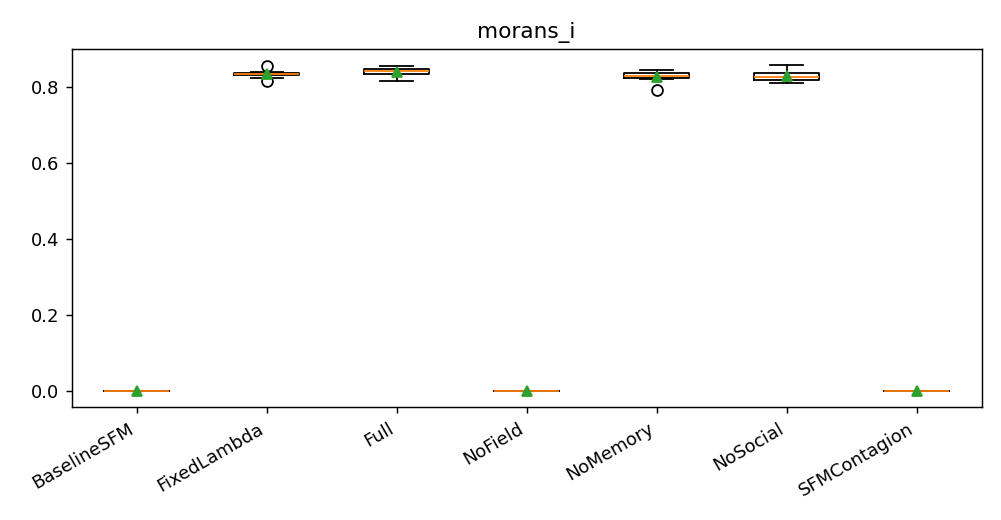
\includegraphics[width=\linewidth]{figures/fig1_morans_i.png}
\caption{Global Moran's $I$ of the affect field by condition (mean, 95\% CI, 10 seeds). Field-on
conditions show strong spatial autocorrelation ($\approx$0.84); field-off conditions are exactly 0.}
\label{fig:morans}\end{figure}

\subsection{The gate is genuinely affect-dependent}
\label{sec:lambda}
The second contribution is affect-gated arbitration: blending a reactive Social-Force action with a
learned PPO correction through a gate
$\lambda = \sigma(\mathrm{raw} + b_0 + k_a\,\ell + k_f\,\phi)$ whose dual-process prior pushes
$\lambda$ toward reactive, System-1 control as affective load $\ell$ rises. For this to be a
meaningful arbitration mechanism rather than a static blend, $\lambda$ must actually co-vary with
affect at runtime. It does: across agents and timesteps the gate tracks affective load with Pearson
$r=0.83$, and a multiple regression of $\lambda$ on the cognitive-state variables attains $R^2=0.67$
with a dominant, positive, standardised load coefficient ($\beta=+0.81$, $p<0.001$)---the
dual-process direction encoded by the prior. The $\lambda$-maps in Fig.~\ref{fig:lambda} make the same
point spatially: the gate field visibly tracks the affect field, shifting toward reactive physics in
the high-affect (red) regions.

This result is best read against the negative finding that motivated the design. A \emph{free} gate,
$\lambda=\sigma(\mathrm{raw})$, with no structural prior, did not discover this relationship: PPO
collapsed it to a near-constant $\lambda\approx0.43$ that was essentially independent of affect
($R^2\approx0.001$). We report this honestly as the central evidence for the structured gate. The
contrast between $R^2\approx0.001$ (free) and $R^2=0.67$ (structured) localises where the
affect-dependence comes from: the \emph{sign and bulk} of the load--$\lambda$ relationship are
imposed by the prior ($k_a>0$, with $b_0$ a physics-dominant bias), which is why we frame the
mechanism as a \emph{structured} gate carrying a \emph{learned residual} rather than as an emergent
discovery. What the policy contributes is the residual variation around that prior---the
$\mathrm{raw}$ term---so the headline $R^2$ should be understood as the dual-process scaffold plus a
learned correction, not as the network spontaneously inferring a dual-process controller.

It is important to be equally explicit about the operating point of this gate. With the
physics-dominant bias the realised blend sits near $\lambda\approx0.94$, i.e.\ heavily weighted toward
the reactive Social-Force action. The arbitration is therefore \emph{measurable but behaviourally
gentle}: the affect-driven modulation of $\lambda$ is real and statistically strong as a relationship,
but it rides on a small dynamic range around a physics-dominant baseline. We quantify this footprint
directly in \S\ref{sec:stress}. We regard this honesty as preferable to the residual-RL convention of
a \emph{fixed} additive sum \cite{johannink2019} or to uncertainty-gated arbitration
\cite{daw2005,lee2014}: the blend here is state-dependent, and the dependence is on affect rather than
on uncertainty, which to our knowledge is novel in crowd simulation---while remaining, in this regime,
a gentle modulation rather than a dominant behavioural switch.

\begin{figure}[t]\centering
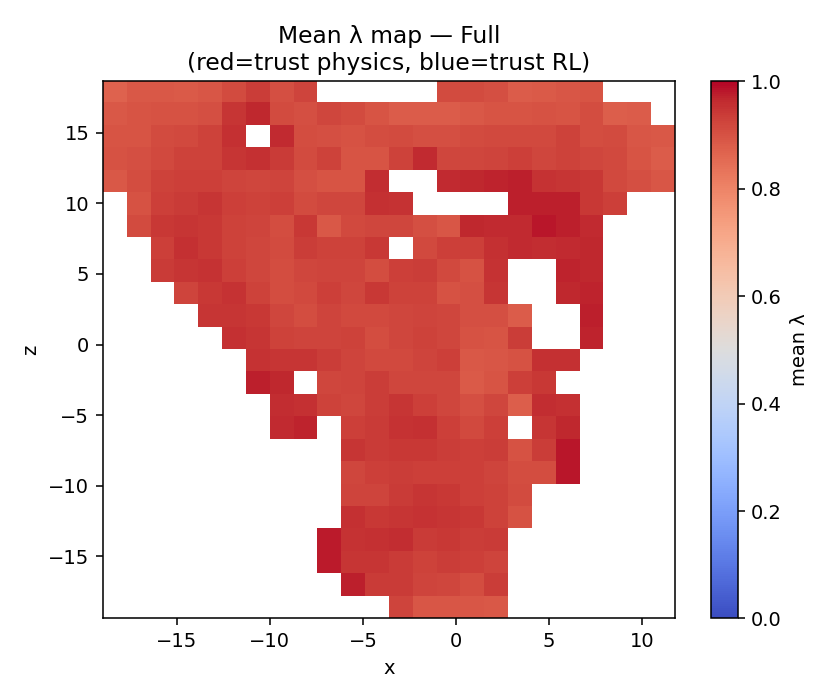
\includegraphics[width=\linewidth]{figures/fig2_lambda_map.png}
\caption{Spatial map of the learned arbitration $\lambda$ (Full). Red: trust reactive physics;
blue: trust the RL correction.}
\label{fig:lambda}\end{figure}

\subsection{The learned controller improves egress}
\label{sec:throughput}
Having established that the field is structured and that the gate is affect-dependent, we ask whether
the learned arbitration is useful as a controller at all. On egress throughput it is: the
RL/arbitration conditions reach $18.8$--$24.1$ goals/run, against $8.6$--$9.6$ for the pure
Social-Force baselines (\texttt{BaselineSFM}, \texttt{SFMContagion})---roughly a $2.5\times$
improvement (Fig.~\ref{fig:throughput}). The gain holds at comparable agent--agent contact rates, so
it does not come from the policy simply pushing harder and trading collisions for speed.

We interpret this as the PPO residual supplying the medium-horizon goal-seeking that a purely
local Social-Force controller \cite{helbing1995} lacks: the reactive base resolves immediate
separation and obstacle repulsion, while the learned correction contributes the longer-horizon
steering toward the egress. This is consistent with the broader RL-locomotion literature
\cite{long2018,chen2017cadrl,everett2018gacadrl}, but our policy adds that decision-making as a
\emph{residual} on top of a stable reactive base rather than replacing the controller wholesale---the
physics-dominant bootstrap ($b_0=\textsc{PhysicsBias}$; see the Discussion) that keeps $\lambda$ near
its reactive operating point without sacrificing throughput. Two qualifications are worth stating up
front. First, the gain is attributable to the presence of the RL correction, not to the affect field:
as \S\ref{sec:stress} shows, adding the field slightly \emph{reduces} throughput. Second, throughput
is measured in a single open $40\times40$ arena with $\sim$20 agents, so the $2.5\times$ figure should
be read as evidence that the learned arbitration is a competent controller in this regime, not as a
claim of universal egress superiority.

\begin{figure}[t]\centering
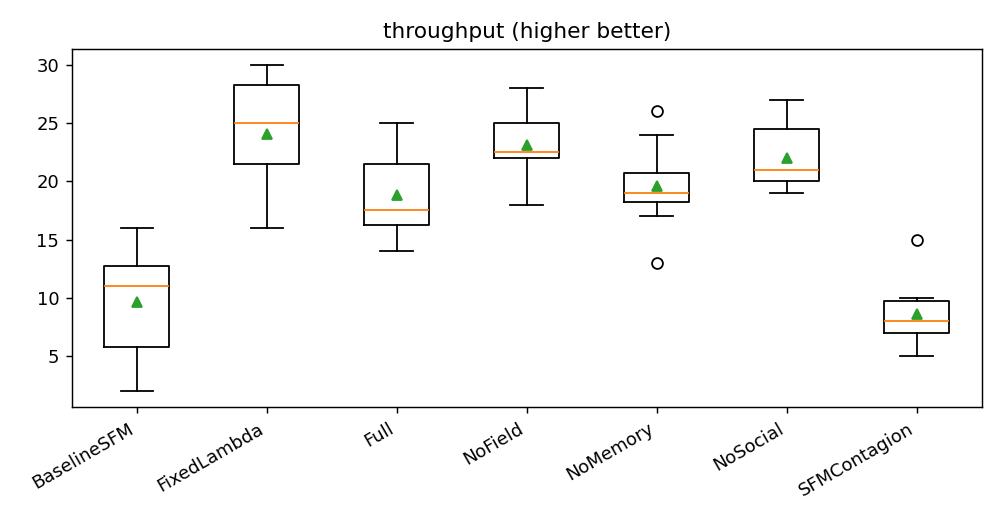
\includegraphics[width=\linewidth]{figures/fig3_throughput.png}
\caption{Egress throughput by condition (mean, 95\% CI, 10 seeds). Learned-arbitration conditions
roughly double the pure Social-Force baselines.}
\label{fig:throughput}\end{figure}

\subsection{Emergent stress-modulated egress}
\label{sec:stress}
The field is not a free performance lever, and it is important not to present it as one. Comparing the
two conditions that differ only in whether the field is active, enabling it slightly \emph{lowers}
throughput (\texttt{Full} $18.8$ vs.\ \texttt{NoField} $23.1$ goals/run) while raising localised
affective load. The mechanism is the intended one: the field concentrates affect in
contiguous high-stress regions (\S\ref{sec:morans}), elevated load nudges $\lambda$ toward reactive
control (\S\ref{sec:lambda}), and through the cognitive-state coupling---affect raises personal space
and modulates desired speed---agents slow down where the field is hot. The net effect is that crowds
\emph{self-impede} in high-affect zones.

This effect should be read at its true magnitude. Because the gate is physics-dominant
($\lambda\approx0.94$), the behavioural footprint of the arbitration is modest: the speed-distribution
divergence between \texttt{Full} and \texttt{FixedLambda} (physics-only with RL present) is only
Jensen--Shannon $\approx0.012$. The stress-modulated slowdown is thus a gentle, localised modulation
of an otherwise physics-driven flow, not a dramatic behavioural switch; the throughput reduction it
produces is correspondingly small.

We read this as a feature rather than a defect: it is a qualitatively correct reproduction of the
real phenomenon whereby panic and crowding impede egress rather than expedite it, emerging from the
field--gate--locomotion coupling rather than being scripted as a rule. It also clarifies the division
of labour between the two contributions. The RL residual is what makes the crowd \emph{fast}
(\S\ref{sec:throughput}); the affect field is what makes the crowd \emph{psychologically plausible},
even at a small throughput cost. A model that only optimised egress would discard the field; a model
that aims to capture collective emotion should accept this trade-off and report it, which is why we
present the throughput reduction openly rather than tuning it away.

\subsection{Agent-drain: the field is an autonomous substrate}
\label{sec:drain}
The second distinguishing property of a stigmergic representation is that the medium has its own
dynamics, independent of the population that wrote to it. We test this directly with an
\emph{agent-drain} protocol: let the field build under normal operation, then at $t=30$\,s remove
\emph{all} agents at once and continue recording the field. If affect were per-agent state propagated
over a neighbour graph, it would read $\approx0$ the instant the agents are gone. Instead the field
persists and relaxes smoothly under its own decay term, falling off exponentially at
$k\approx0.34\,\mathrm{s}^{-1}$ with a half-life of $\approx$2.0\,s; $52\%$ of the drain-time affect
remains $2$\,s later and $\sim$18\% remains at $+5$\,s (Fig.~\ref{fig:drain}).

The quantitative agreement is the load-bearing part. The measured decay rate $k\approx0.34\,\mathrm{s}^{-1}$
matches the configured $-k\phi$ term ($k=0.35$) of the reaction--diffusion dynamics to within
estimation noise, which establishes that the post-drain signal is genuinely the field obeying its own
governing equation---not a measurement artefact or residual agent state---and that its relaxation is
\emph{independent of agent count}. This is the temporal counterpart to the spatial result of
\S\ref{sec:morans}: where Moran's $I$ shows the field has structure no pairwise model can represent,
the agent-drain shows the field has memory no pairwise model can hold, since a neighbour-graph update
\cite{durupinar2008,bosse2013ascribe,tsai2011escapes,vanhaeringen2023} has no state once its carriers
are removed. Together, spatial structure and population-independent persistence are exactly the two
properties that justify calling the representation a field rather than a faster contagion rule.

\begin{figure}[t]\centering
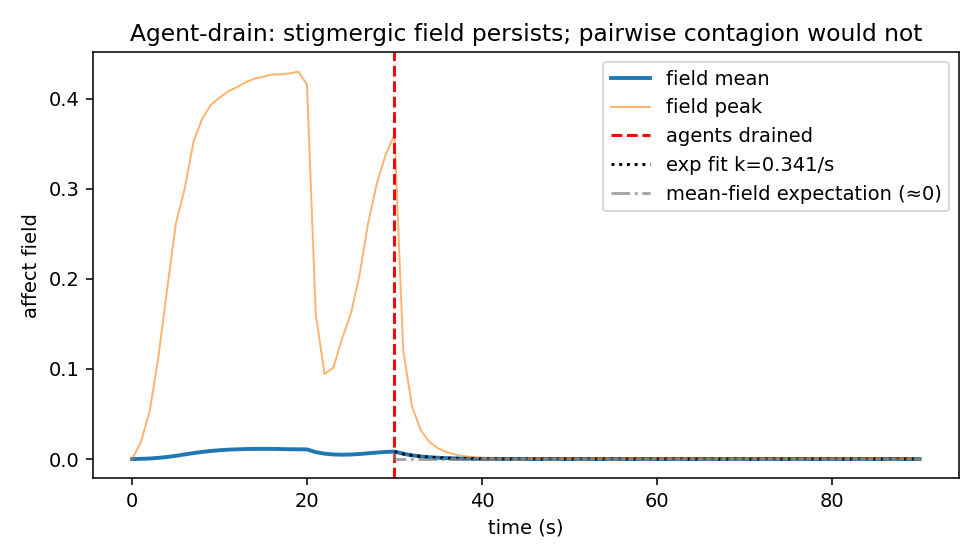
\includegraphics[width=\linewidth]{figures/fig4_agent_drain.png}
\caption{Agent-drain test: affect-field mean over time. After all agents are removed at $t=30$\,s
the field persists and decays at its own rate---not to zero instantly as a pairwise model would.}
\label{fig:drain}\end{figure}

\subsection{Fundamental diagram (dense corridor)}
\label{sec:fd}
Spatial structure, affect-dependence, and substrate autonomy concern the novel mechanisms; the
fundamental diagram asks the orthogonal question of whether the underlying locomotion is physically
plausible against published pedestrian data. In a periodic corridor with position-based contact
resolution, measuring realised net forward speed over the density range $0.17$--$4.33$~ped/m$^2$, the
free-flow speed is $1.38$~m/s, essentially matching the Weidmann reference value $v_0=1.34$~m/s. As
density rises, speed falls to $\sim$0.48~m/s at $1.67$~ped/m$^2$, consistent with the empirically
reported $\sim$0.5--0.7~m/s in the $1$--$1.7$~ped/m$^2$ band. The congested branch up to
$\sim$1.7~ped/m$^2$ therefore matches the published fundamental diagram in both \emph{shape} and
\emph{magnitude} (Fig.~\ref{fig:fd}), not merely qualitatively---which is the appropriate sanity check
for a Social-Force locomotion layer \cite{helbing1995} and gives independent grounding to the
throughput and stress results that depend on it. We stress that this is agreement with an
\emph{aggregate} empirical fundamental diagram, not trajectory-level validation against real
crowd data, which we have not yet performed.

We are explicit about where this breaks down. Above $\sim$1.7~ped/m$^2$ the model shows a mild speed
\emph{recovery} (from $\sim$0.48 up to $\sim$0.67~m/s) instead of the continued collapse toward
jamming that real crowds exhibit. We attribute this to the simplified position-based contact model,
which does not enforce the velocity-coupled volume exclusion that produces gridlock at extreme
density; a velocity-based scheme such as ORCA/RVO would be required to capture that regime. We report
the recovery rather than truncating the plot at $1.7$~ped/m$^2$ because the honest claim is bounded:
the locomotion reproduces the published fundamental diagram up to moderate-to-high density, and the
extreme high-density branch is a known limitation, not a captured behaviour.

\begin{figure}[t]\centering
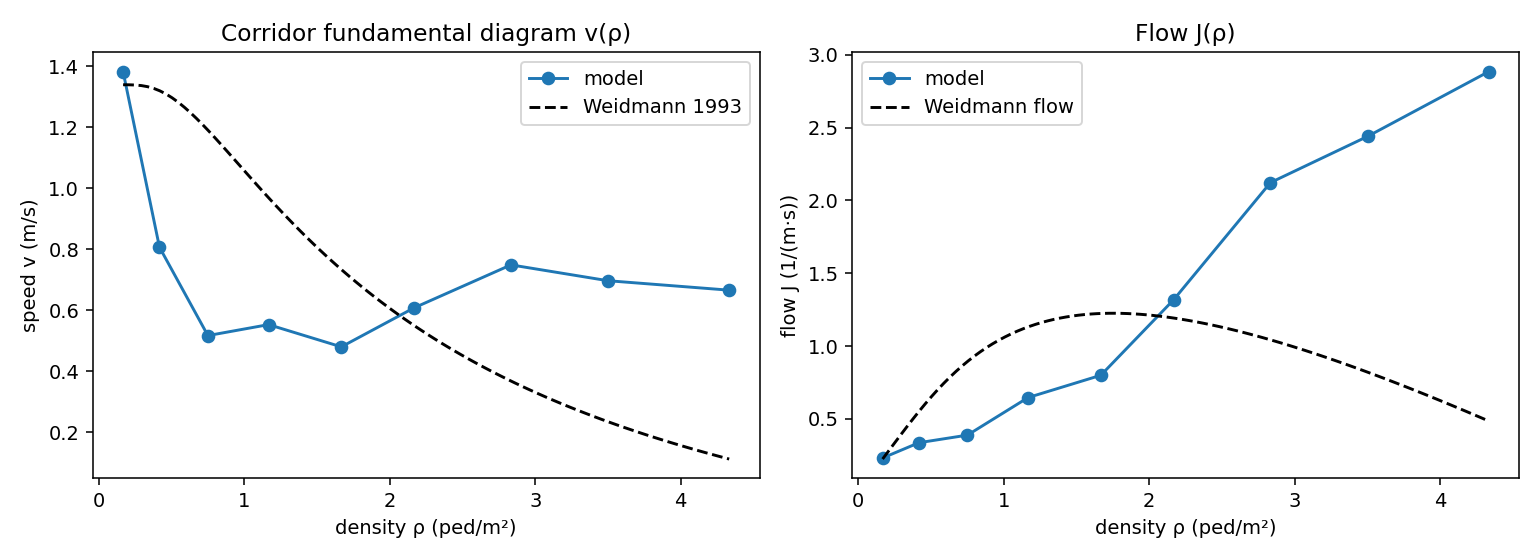
\includegraphics[width=\linewidth]{figures/fig5_fundamental_diagram.png}
\caption{Corridor fundamental diagram: model $v(\rho)$ and flow $J(\rho)$ against the Weidmann
reference. Free speed and the congested drop match the published empirical curve up to
$\sim$1.7~ped/m$^2$; above that the model shows a mild speed recovery rather than jamming.}
\label{fig:fd}\end{figure}

\subsection{Field vs.\ pairwise contagion (head-to-head)}
\label{sec:headtohead}
Finally, the ablation is constructed so that the field-vs-pairwise comparison is matched rather than
confounded. \texttt{Full} adds the stigmergic field on top of pairwise contagion, while
\texttt{NoField} retains the pairwise contagion but removes the field. \texttt{NoField} is therefore
\emph{literally} a pairwise-contagion model running in the identical environment, under the identical
shared policy and the identical seeds---the only difference between the two conditions is the
representational choice under test. On that matched pair, the field condition yields Moran's
$I=0.84$ while the pairwise condition yields exactly $0$ ($p<0.001$, $\delta=-1.0$), and the
agent-drain persistence of \S\ref{sec:drain} holds only for the field.

This design is what licenses the central claim of the first contribution as a controlled result
rather than a cross-model comparison. Because environment, policy, and seeds are held fixed, the two
properties that separate the conditions---spatial emotional structure (\S\ref{sec:morans}) and
population-independent memory (\S\ref{sec:drain})---can be attributed to the field representation
itself and not to incidental differences in setup. These are precisely the two properties that the
neighbour-graph contagion line of work
\cite{durupinar2008,durupinar2016,bosse2013ascribe,tsai2011escapes,vanhaeringen2023} cannot exhibit,
so the head-to-head establishes, on matched runs, that the stigmergic affect field is a
distinct---not merely a reparameterised---model of collective emotion.

\subsection{Causal interpretability of $\lambda$ (clamp-and-probe)}
To test whether $\lambda$ \emph{causally} drives behaviour rather than passively correlating with
geometry, we clamp $\lambda$ to fixed values at inference (all features Full) and sweep it (10 seeds).
Egress throughput rises monotonically with $\lambda$---0.1 goals at $\lambda=0$ to 12.3 at $\lambda=1$
(range 12.2): at $\lambda=0$ (pure RL residual) agents are nearly immobile (speed 0.09~m/s, elevated
stress and contacts) because the policy learned the RL term as a small correction atop physics, while
as $\lambda\to1$ physics-driven goal-seeking dominates (Fig.~\ref{fig:probe}). Forcing $\lambda$ thus
systematically and causally changes behaviour, confirming the gate is a genuine control variable, not
a geometry proxy. The learned gate ($\lambda\approx0.94$) operates near the physics end (throughput
9.6), slightly below pure physics (12.3): honestly, the learned arbitration does not maximise egress;
it selects a physics-dominant operating point with a small learned admixture, consistent with the
modest behavioural footprint reported above.


\begin{figure}[t]\centering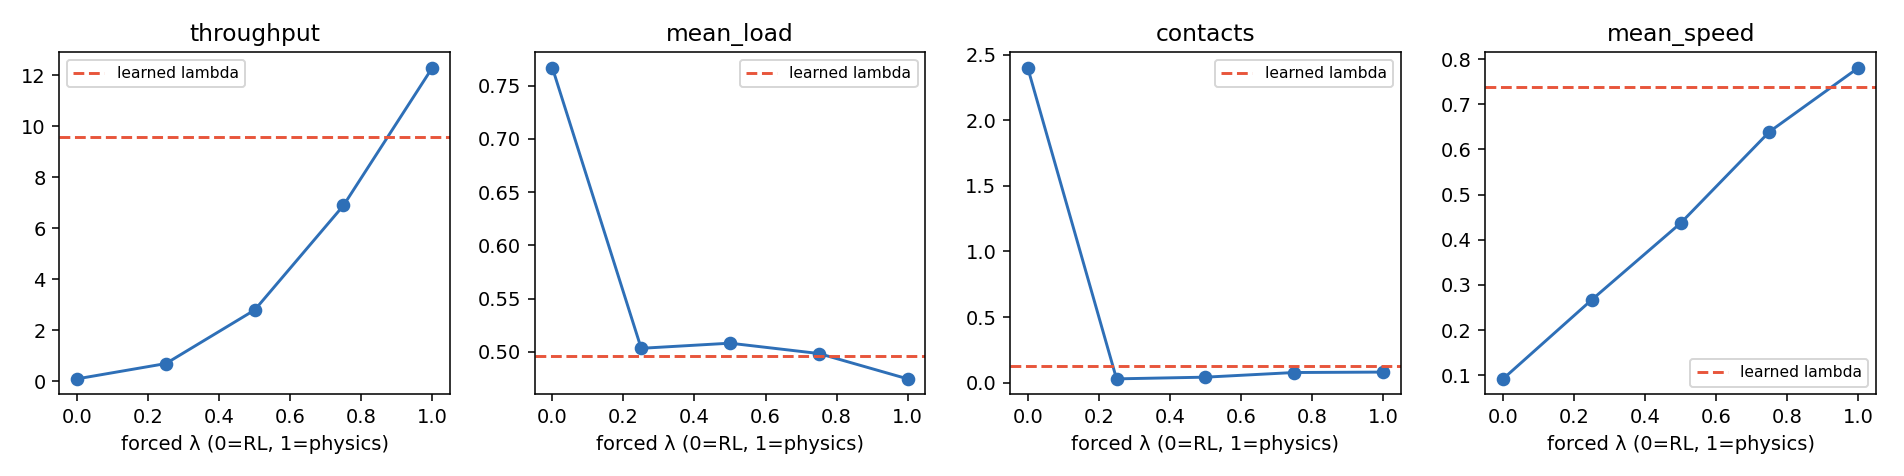
\includegraphics[width=\linewidth]{figures/fig7_lambda_probe.png}
\caption{Clamp-and-probe: behaviour vs.\ forced $\lambda$ (mean, 10 seeds). Throughput rises monotonically with $\lambda$ (0.1$\to$12.3 goals), causal evidence that the gate drives behaviour; the learned gate (dashed) sits near the physics end.}\label{fig:probe}\end{figure}


\section{Generalisation, Coordination, and Two Further Mechanisms}
The results so far come from the single open arena of the core ablation. This section reports six
additional studies: that the field's spatial signature \emph{generalises} across layouts
(\S\ref{sec:gen}); that, given a decision channel, the field acts as a \emph{communication-free
coordination substrate} (\S\ref{sec:coord}); two mechanisms we had listed as future work---a
precision-based gate (\S\ref{sec:prec}) and an anisotropic flow-coupled field
(\S\ref{sec:aniso})---which we now evaluate, the second as an honest negative; that collective
panic in the affect+field core has the structure of a \emph{phase transition} (\S\ref{sec:phase}); and,
inverting the field's role, that it can serve as a crowd-steering \emph{actuator}---though naive central
control of it is beaten by self-organisation (\S\ref{sec:actuator}). Two caveats apply
throughout: the procedural-layout experiments use the locomotion/affect stack \emph{without} the RL
policy (so $\lambda$ takes its hand-designed fallback), and they route agents through doors with an
explicit waypoint path because the local controller has no global planner; both are stated where they
bear on a claim.

\subsection{Generalisation across layouts}
\label{sec:gen}
To test whether the field's spatial structure is an artefact of the open square, we re-ran the
field-on vs.\ field-off contrast across six RiMEA-style benchmark layouts~\cite{rimea}---open square,
single bottleneck, two-exit room, bidirectional counter-flow, a $90^\circ$ corner, and a four-way
crossing (Fig.~\ref{fig:layouts}). In \emph{every} layout the field produces strong spatial
autocorrelation of affect (Moran's $I$ between $0.87$ and $0.92$) while the matched pairwise-only
condition is exactly $0$, with Cliff's $\delta=+1.0$ in all six (Fig.~\ref{fig:scenarios}). The
result of \S\ref{sec:morans} is therefore not geometry-specific: the reaction--diffusion substrate
knits deposits into contiguous emotional regions regardless of the obstacle layout. Equally
informative is what does \emph{not} generalise into a behavioural effect: across the same six layouts
the field-on and field-off conditions are statistically indistinguishable on egress, mean speed, and
peak density. This is the multi-layout confirmation of the core finding---the field's footprint is on
the \emph{affective structure} of the crowd, not on its low-level locomotion, consistent with the
physics-dominant gate (\S\ref{sec:stress}).

\begin{figure}[t]\centering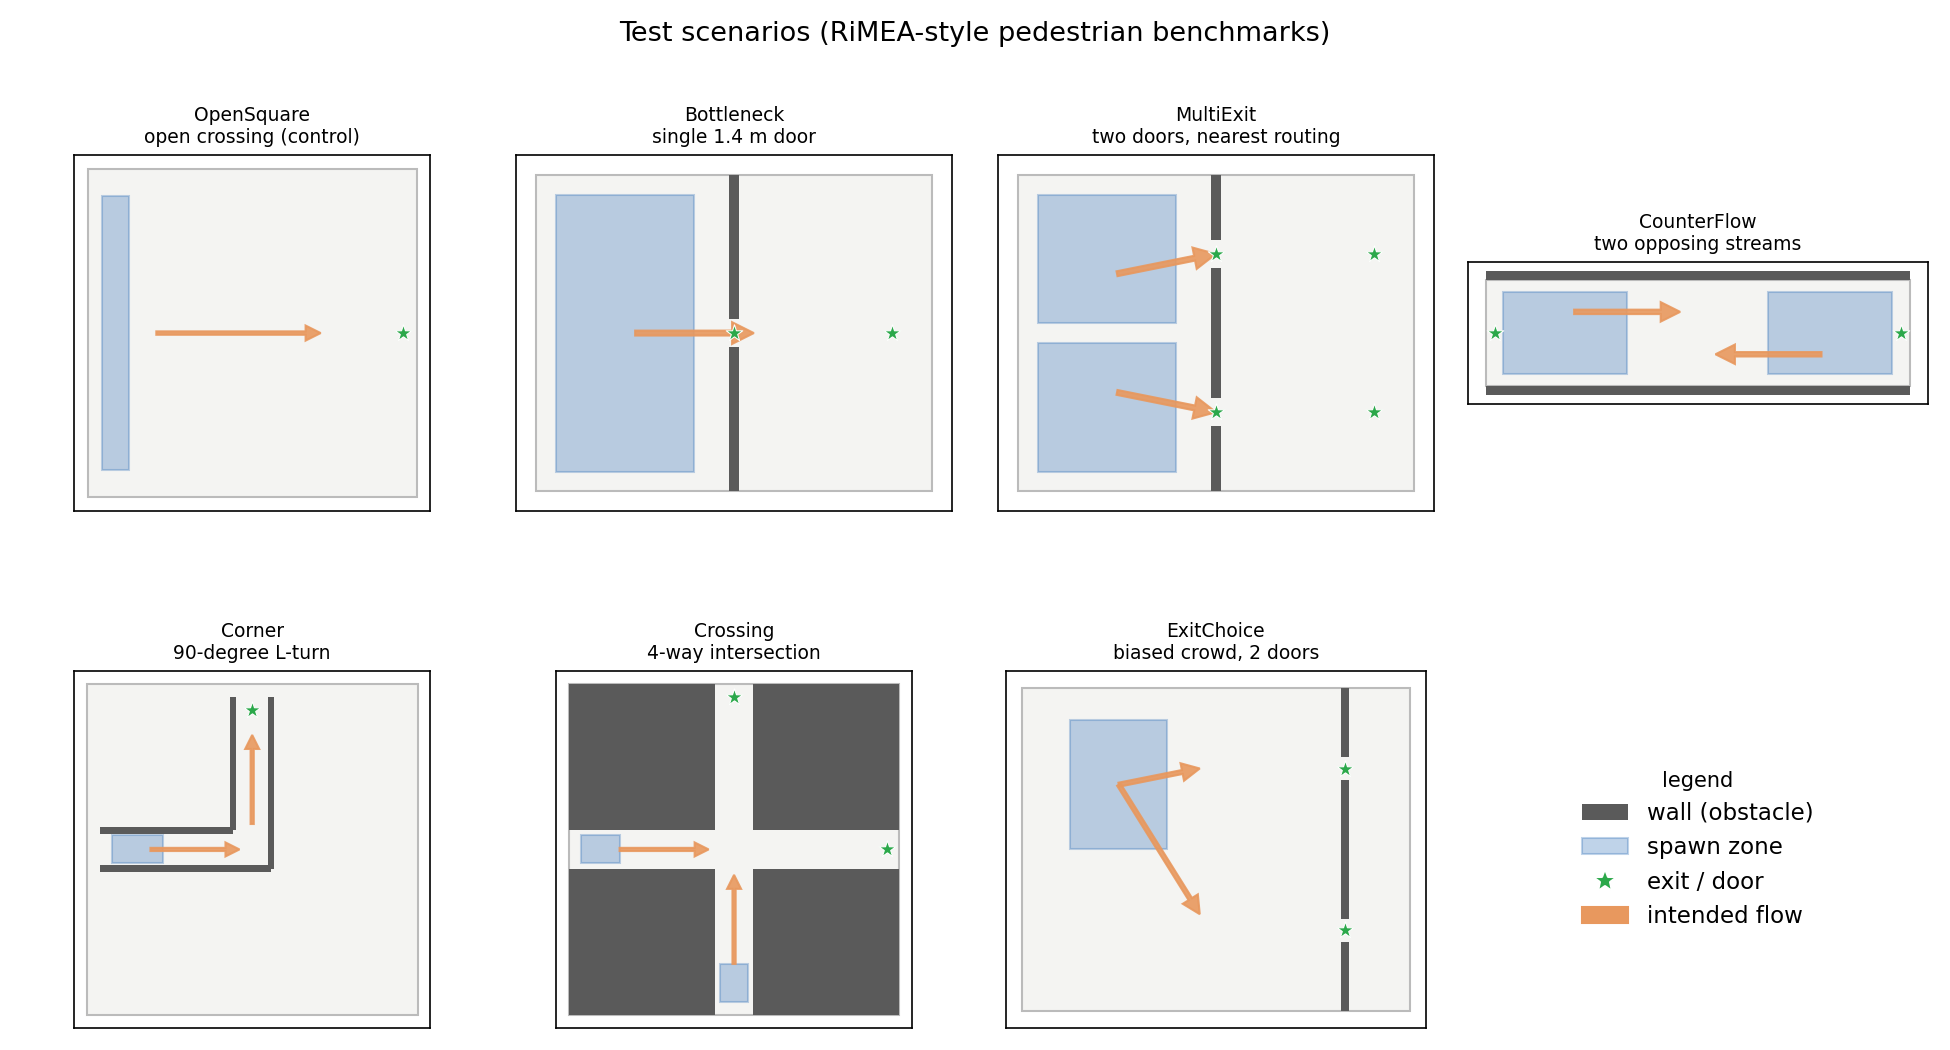
\includegraphics[width=\linewidth]{figures/fig12_scenario_layouts.png}
\caption{The six RiMEA-style test layouts (walls grey, spawn zones blue, exits green, intended flow
arrows). The affect+locomotion stack is identical across all; only geometry varies.}
\label{fig:layouts}\end{figure}

\begin{figure}[t]\centering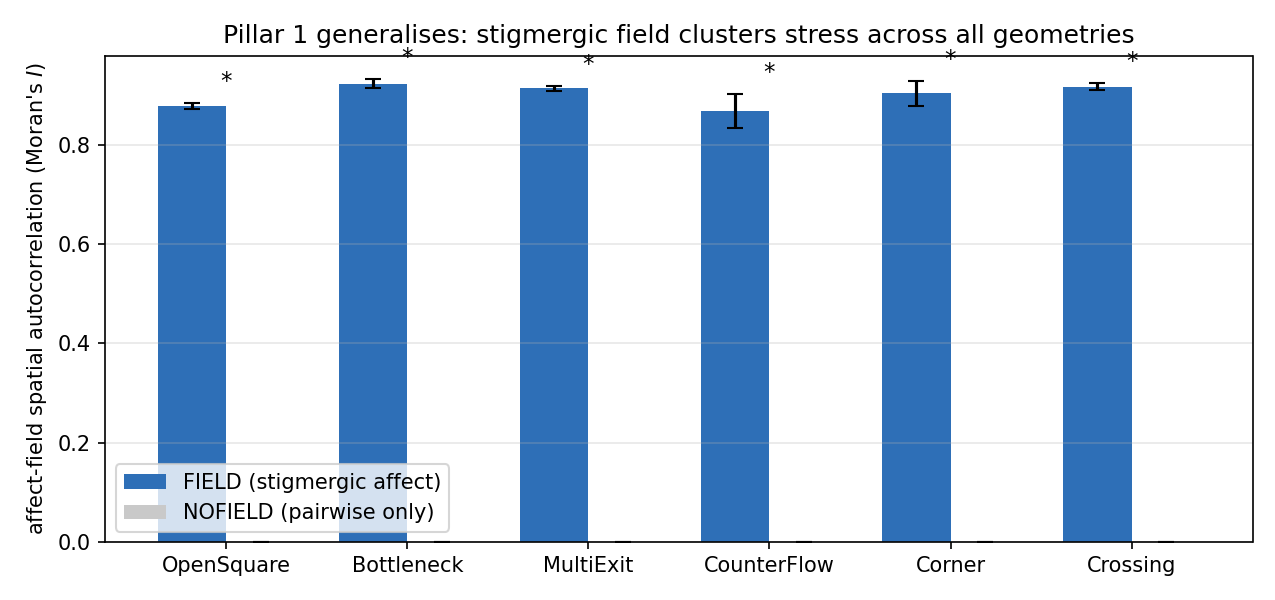
\includegraphics[width=\linewidth]{figures/fig9_scenarios_moransi.png}
\caption{Field spatial autocorrelation generalises: Moran's $I$ is significantly positive
(FIELD) in all six layouts and exactly $0$ for the pairwise baseline (NOFIELD); $\delta=+1.0$ each
(${}^{*}\,p{=}0.032$, the floor for the seed count).}
\label{fig:scenarios}\end{figure}

\subsection{The field as a communication-free coordination substrate}
\label{sec:coord}
The core ablation forced each agent's exit, so the field could not influence route choice---the very
channel in which a spatial affect signal should matter most. We therefore opened that channel: in a
multi-exit room the crowd is spawned biased toward one door, and we compare a \emph{Baseline} that
routes each agent to its nearest (lowest-cost) door against a \emph{FieldRoute} rule that subtracts an
affect penalty from each door's score, $\text{score}(d) = -\text{dist}(d) - k_\Phi\,\Phi(d)$, so
agents avoid the door whose queue has grown emotionally hot. Both conditions run the \emph{identical}
field; only whether route choice reads it differs---and crucially, agents share no messages, sensing
only the environmental field, so any redistribution is stigmergic~\cite{theraulaz1999stigmergy}
coordination. Across three layouts (symmetric two-exit, three-exit, and a near/far pair), $10$ seeds
each, FieldRoute lowers the max-exit share---i.e.\ balances the doors---in every case: two-exit
$0.97\!\to\!0.77$ ($p{=}0.016$, $\delta=-0.51$), near/far $0.99\!\to\!0.86$ ($p{=}0.001$,
$\delta=-0.74$), three-exit $0.79\!\to\!0.65$ ($p{=}0.069$, borderline); mean speed rises in all three
($p\le0.002$). The mechanism is visible in raw door usage: in the near/far layout the Baseline sends
essentially no one to the far exit ($0.1$ of $\sim$10 evacuees) while FieldRoute sends $4.3$
(Fig.~\ref{fig:coord}). Most consequentially, the near/far layout---the one that reproduces the lethal
``everyone crowds the near exit'' pattern of real disasters---is also where redistribution
\emph{pays}: FieldRoute evacuates $12.4$ agents in $60$\,s against the Baseline's $8.0$ ($p{=}0.037$,
$\delta=+0.48$), a $\sim$55\% gain. In the symmetric two- and three-exit layouts the balancing does
not significantly change total throughput, which we report as the honest boundary of the effect: a
shared affect field can break a pathological single-exit commitment without central control, but
balancing only helps net egress when an exit was being genuinely wasted.

\begin{figure}[t]\centering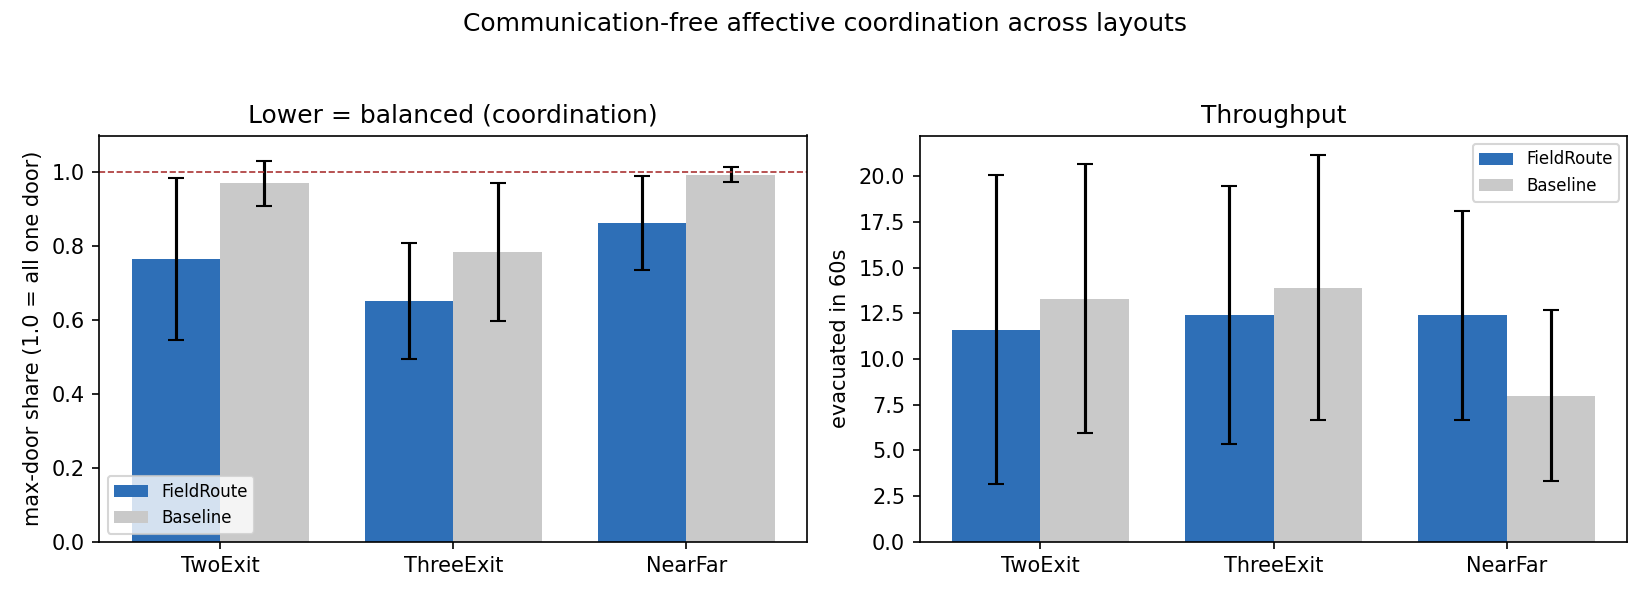
\includegraphics[width=\linewidth]{figures/fig13_coordination.png}
\caption{Communication-free coordination across three multi-exit layouts. \emph{Left}: max-exit
share (lower $=$ better balanced); FieldRoute balances every layout. \emph{Right}: throughput;
in the near/far layout FieldRoute also evacuates significantly more agents.}
\label{fig:coord}\end{figure}

\subsection{An inference-time precision gate}
\label{sec:prec}
We had proposed replacing the fixed affect bias with a \emph{precision} signal in the spirit of
uncertainty-weighted arbitration~\cite{daw2005,lee2014}. We implement a tractable, inference-time
version that needs no retraining: the agent's behavioural ``stuckness'' $u_i$ (the same uncertainty
signal of Eq.~\eqref{eq:load_in}) is read as the inverse precision of the reactive controller, and is
subtracted from the gate, $\lambda_i = \sigma(r + b_0 + k_a\ell_i + k_f\phi_i - k_p\,u_i)$, so that
when physics is failing (the agent is stuck, $u_i$ high) control shifts toward the deliberative RL
residual. Running the trained policy in the arena with the gate off vs.\ on ($k_p=4$), the gate does
what it is designed to: mean $\lambda$ drops $0.95\!\to\!0.85$ and the RL share of acceleration rises
($1.8\%\!\to\!5.8\%$), and this \emph{reduces} stuck-states---mean uncertainty falls $\sim$24\%
($0.246\!\to\!0.186$) and the fraction of stuck agent-steps falls $\sim$22\%. The trade-off is a
$\sim$10\% drop in mean speed ($0.82\!\to\!0.73$\,m/s): deferring to a residual trained only as a
small correction is more cautious than goal-seeking physics, consistent with the dual-process
prediction that the deliberative system is slower but escapes traps the reactive one falls into. We
report this as a \emph{directional} result (a single matched run per condition, not a multi-seed
significance claim): the precision gate is a working, retraining-free arbitration mechanism whose
benefit is reduced stuck-time rather than raw speed.

\subsection{Anisotropic flow-coupled diffusion: an honest negative}
\label{sec:aniso}
Finally we evaluate the anisotropic, flow-coupled field we had proposed---one whose affect is advected
along the local crowd-flow direction rather than diffusing isotropically, predicting that emotion
should spread preferentially \emph{downstream}. At the operator level the scheme is correct: injecting
a tracer pulse under a uniform flow and stepping the discretised update advects the field's centroid
$\sim$6 cells downstream in $2$\,s, versus $0$ with the flow off (Fig.~\ref{fig:tracer}). But the
\emph{prediction we set out to test}---that directional Moran's $I$ would be larger along the flow
axis than across it---is \emph{not} supported in the agent simulation. In a square arena with uniform
flow, the difference-of-differences (along-minus-across, advection-on minus advection-off) is
$-0.037$ (Mann--Whitney $p{=}0.96$, $\delta=-0.20$): advection does \emph{not} add detectable
directional anisotropy. The reason is a confound we can state precisely: agents moving along the flow
already deposit affect along their trajectories, so the field is flow-aligned even with advection
off, and the global directional statistic cannot separate transport from trajectory-deposition.
Advection's measurable effect is instead an \emph{isotropic} increase in overall field coherence
($+0.25$ mean Moran's $I$). We report this as a negative result---the operator transports as designed,
but the chosen observable does not identify it---which scopes the correct future test toward a
tracer/pulse-displacement metric rather than aggregate autocorrelation.

\begin{figure}[t]\centering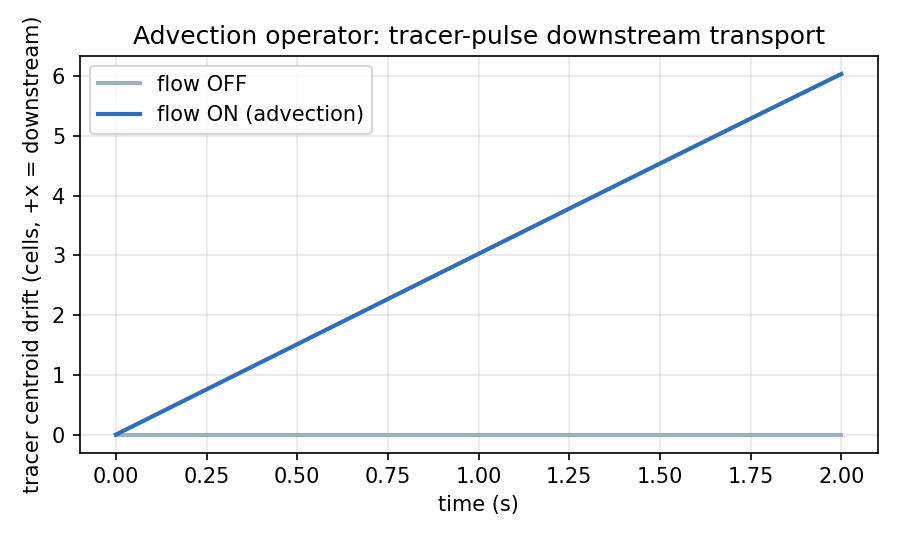
\includegraphics[width=0.85\linewidth]{figures/fig8b_advection_tracer.png}
\caption{Operator-level check of the flow-coupled field: a tracer pulse's centroid advects
$\sim$6 cells downstream in $2$\,s with flow on and not at all with flow off---the operator transports
correctly, even though its directional signature is not recoverable from aggregate Moran's $I$
in the agent simulation.}
\label{fig:tracer}\end{figure}

\subsection{Collective panic as a phase transition}
\label{sec:phase}
The affect field closes a positive feedback loop: stressed agents \emph{deposit} affect (deposit
$\propto$ load) and the field \emph{drives} affect (load $\propto$ field pressure, with gain $g_\phi$).
Whenever a deposit--diffuse--decay medium is coupled to its own sources this way one expects a
threshold---below a critical feedback the calm state is stable, above it the loop runs away---so we
ask whether collective panic in our model is, structurally, a phase transition. We test this in a
faithful reduced model (the affect+field core in isolation, agents static) and in the full Unity model
(complete locomotion + affect stack, no RL, on a \emph{periodic/torus} arena so density is uniform with
no wall-induced crowding). The order parameter is the steady-state mean affective load
$M=\langle\ell\rangle$; we also track a finite-size susceptibility (the temporal fluctuation of $M$) and
the fraction of agents with $\ell>0.5$.

Both models show a sharp calm$\to$panic transition. Sweeping crowd density in the full model, $M$ jumps
from $\approx0$ (calm) to $\approx1$ (panic) across a narrow band and the susceptibility \emph{peaks at
the critical density} $\rho^\star\approx0.06$~ped/m$^2$ (Fig.~\ref{fig:phase}, left)---the textbook
signature of a critical point. Sweeping the field$\to$affect gain $g_\phi$ at fixed density reproduces
the same onset at a low critical gain, and the reduced model predicts the same structure
($\rho^\star\!\sim\!0.1$), so the transition is a property of the affect--field coupling rather than of
any one implementation.

A second observation carries the real-world reading. \emph{Without} a stabiliser the full model
saturates to panic at \emph{every} tested density, even sparse ones: the stigmergic feedback alone is
strongly self-amplifying. Re-introducing the model's calming term (familiarity-driven relief) restores
a finite calm phase and exposes the transition, and a sweep of the calming strength behaves as a
\emph{reassurance threshold}---but at a density well above $\rho^\star$ even near-maximal reassurance
only partly rescues the crowd (Fig.~\ref{fig:phase}, right). The control reading is then sharp:
collective panic has a \emph{tipping point}; reassurance can hold a near-critical crowd in the calm
phase, but once the crowd is well past $\rho^\star$ the only remedy is to reduce density. This is a
plausible mechanism for the suddenness and near-irreversibility of real crowd disasters and is
consistent with the empirically reported onset of ``crowd turbulence'' above a critical
density~\cite{helbing2007turbulence}.

We are explicit about the limits. The absolute critical density here ($\rho^\star\!\approx\!0.06$~ped/m$^2$)
is far below the $\sim$6~ped/m$^2$ at which real crowd turbulence sets in, because the milling
reduced/torus setups omit the movement- and landmark-driven calming that would raise the threshold; the
\emph{qualitative} structure---a sharp transition with a susceptibility peak, and a stabiliser that sets
the threshold---is the result, not the numeric value. Mapping the true critical surface and using it as a
design target for keeping crowds sub-critical motivates an \emph{active control} of the field, which we
turn to as the principal direction for future work.

\begin{figure}[t]\centering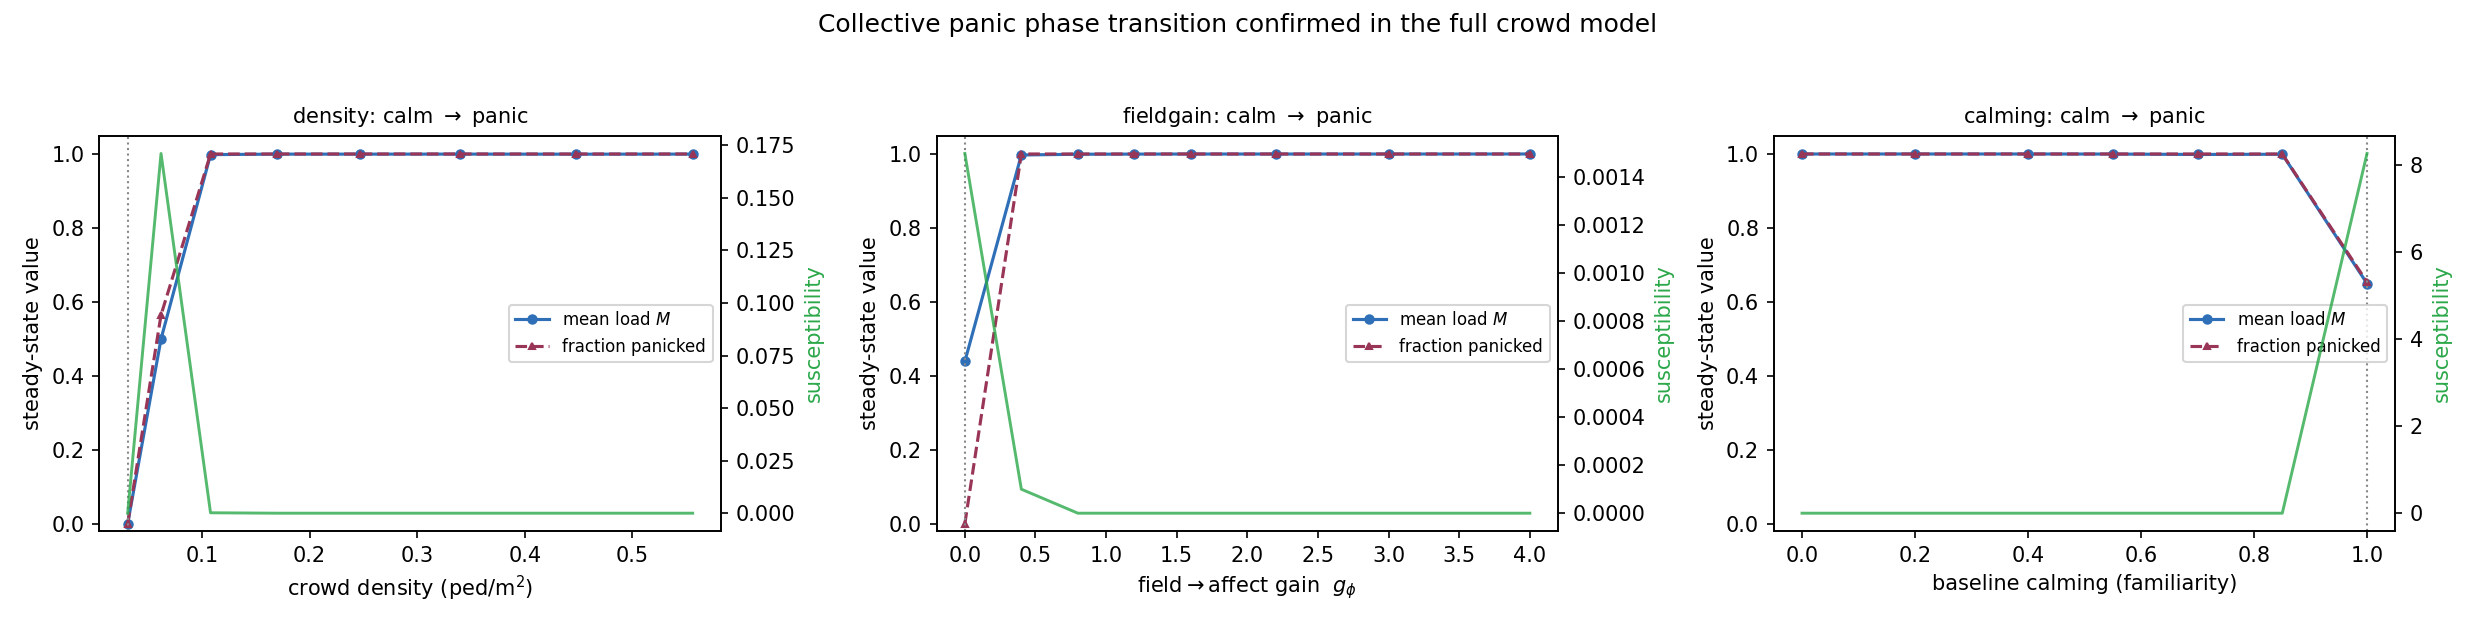
\includegraphics[width=\linewidth]{figures/fig15_phase_unity.png}
\caption{Collective panic as a phase transition (full crowd model, periodic arena). \emph{Left}:
sweeping crowd density, mean affective load tips sharply from calm to panic and the susceptibility
(green) peaks at the critical density $\rho^\star\approx0.06$~ped/m$^2$. \emph{Right}: at a super-critical
density, baseline calming (reassurance) breaks the panic state only near its maximum---once well past
$\rho^\star$, reassurance alone cannot rescue the crowd.}
\label{fig:phase}\end{figure}

\subsection{Active control of the field: a steering actuator, but self-organisation wins}
\label{sec:actuator}
The phase transition (\S\ref{sec:phase}) frames a control goal---keep the crowd sub-critical and balance
its load across exits---and inverts the field's role from something agents \emph{read} to something an
external safety controller \emph{writes}, making the affect field a candidate \emph{actuator} for adaptive
evacuation guidance (dynamic signage, lighting, or announcements that modulate how attractive each route
feels). We test this in the near/far room (one near, one far exit; crowd biased toward the near door) with
four conditions: \texttt{NoControl} (route to the nearest door), \texttt{SelfField} (agents route
field-aware on their own deposits---the self-organised coordination of \S\ref{sec:coord}), and two external
controllers that deposit affect to discourage the over-used door---\texttt{ActuatorNaive} (open-loop: heat
the busy door) and \texttt{ActuatorCL} (closed-loop: heat the busy door, \emph{cool} the quiet one, with a
deadband), the latter run with a softened field--route coupling and a gentle proportional gain.

The actuator unambiguously \emph{steers}: external writing raises far-exit usage from $2.0$ (NoControl) to
$15.1$ agents (ActuatorCL), Cliff's $\delta=0.95$, $p<0.001$---confirming that writing to the crowd's own
stress signal redirects it. But it does not \emph{balance}: across all three controllers (open-loop,
closed-loop, and the soft-coupled gentle variant) the actuator \emph{over-steers}, flipping the entire
crowd to the far door (max-exit share $=1.0$) and \emph{underperforming} decentralised self-organisation on
both balance (SelfField $0.81$ vs.\ $1.0$) and throughput (evacuated: SelfField $21.3\!\approx\!$NoControl
$20.0 >$ ActuatorCL $15.1 >$ ActuatorNaive $12.0$; Fig.~\ref{fig:actuator}). The cause is a \emph{herding
instability}: agents re-choosing against a shared, slowly-decaying field swing together rather than
splitting, so a global ``discourage the busy door'' policy can only flip the crowd, not partition it.

We report this honestly as an open-problem result, not a control success. Two things are established: the
stigmergic field is a genuine, powerful crowd-steering actuator; and \emph{naive central control of it is
beaten by decentralised self-organisation}---a concrete instance of the broader principle that
self-organised systems can outperform blunt top-down control. Effective active control of an affective
field is therefore non-trivial: it must avoid driving the crowd into a synchronised over-correction, which
points to desynchronised, predictive, or per-agent control as the necessary next step. The caution transfers
directly to real adaptive guidance---a blunt ``push everyone away from the busy exit'' policy over-corrects
and merely relocates the jam.

\begin{figure}[t]\centering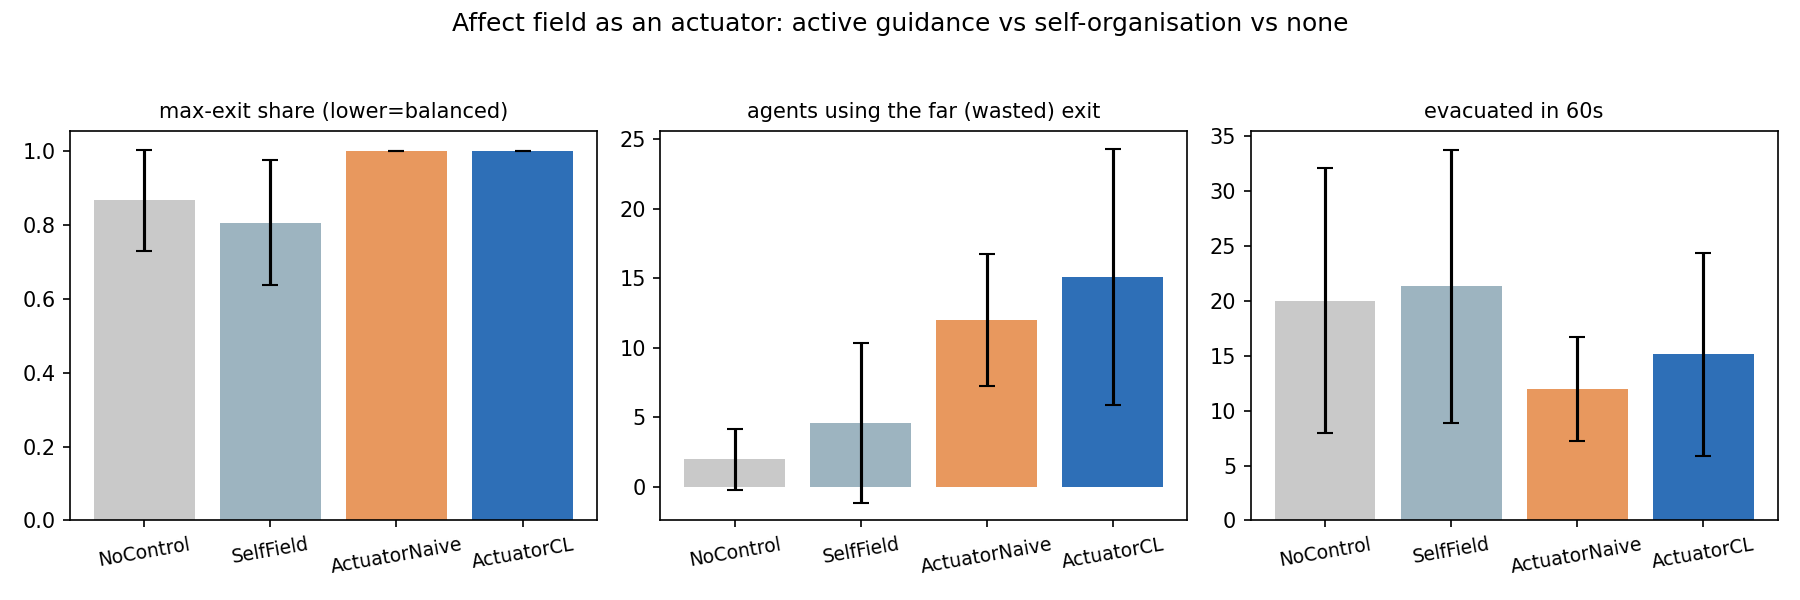
\includegraphics[width=\linewidth]{figures/fig16_actuator.png}
\caption{Affect field as an actuator (near/far room). The external controller steers the crowd to the far
exit (far-exit usage, centre) but \emph{over-steers}: max-exit share returns to $1.0$ (left) and throughput
(right) falls below decentralised self-organisation (\texttt{SelfField}). Naive central control of the
field is beaten by self-organisation.}
\label{fig:actuator}\end{figure}

\section{Discussion and Limitations}
\subsection{A measurable but behaviourally modest arbitration}

The affect-gated arbitration scheme is best understood as a controlled perturbation of an otherwise physics-driven controller rather than a wholesale replacement of it. By construction the gate carries a strong physics-dominant bias ($b_0 = 2.0$), so even with the learned residual and the affect/field terms active, the effective blend coefficient settles near $\lambda \approx 0.94$ in the \emph{Full} condition. The behavioural consequence is exactly what one would predict from that operating point: the speed-distribution divergence between \emph{Full} and \emph{FixedLambda} is only Jensen--Shannon $\approx 0.012$ (Fig.~\ref{fig:lambda}). We read this as a genuine but small footprint. The arbitration \emph{does} move behaviour in a measurable, repeatable direction, but its magnitude is gentle because the system spends most of its time deep in the physics-dominant regime where the corrective force $u_{\mathrm{RL}}$ is heavily down-weighted. We deliberately resist the temptation to report this divergence as a headline effect; it is a small number and we present it as such.

This exposes a design tension we did not fully resolve and want to state plainly: there is a trade-off between \emph{navigational stability} and \emph{behavioural impact} that is governed by $b_0$. A large $b_0$ keeps the Social-Force controller in charge, which is what makes locomotion stable, collision-aware, and reliably goal-reaching --- the same property that underlies the throughput gains of the RL/arbitration conditions ($18.8$--$24.1$ goals/run versus $8.6$--$9.6$ for the pure-SFM baselines, roughly $2.5\times$; Fig.~\ref{fig:throughput}). But that same large $b_0$ is precisely what compresses the dynamic range of $\lambda$ and limits how far affect can bend the trajectory. A smaller $b_0$ would hand more authority to $u_{\mathrm{RL}}$ and to the affect/field terms, plausibly producing a larger behavioural signature, at the cost of the bootstrap stability that the physics-dominant prior buys us during training. We chose the stable end of that spectrum for this study, and the modest arbitration footprint is the honest price of that choice rather than a flaw to be papered over. Quantifying the $b_0$--impact frontier --- how much behavioural divergence one can purchase per unit of lost stability --- is a concrete and worthwhile direction we leave open.

\subsection{Designed versus learned gating}

A central honesty point concerns \emph{where the affect-dependence of $\lambda$ comes from}. Our gate is structured: $\lambda = \sigma(\text{raw} + b_0 + k_a\,\text{load} + k_f\,\text{fieldPressure})$ with $k_a, k_f > 0$ baked in as a dual-process prior, so that higher affective load and higher field pressure push the blend toward the reactive, System-1 physics response. This means the strong empirical relationship we report --- regression $R^2 = 0.67$, standardized load coefficient $\beta = +0.81$ ($p < 0.001$), and $\lambda$--load Pearson $r = 0.83$ --- is \emph{partly by construction}. We are explicit that this is a structured prior carrying a learned residual, not an emergent discovery of dual-process control from reward alone.

We motivate the structured form with a genuine negative result rather than asserting it on aesthetic grounds. When we instead let the gate be \emph{free}, $\lambda = \sigma(\text{raw})$, with no affect terms and no bias, the policy converged to a near-constant $\lambda \approx 0.43$ that was effectively independent of affect (regression $R^2 \approx 0.001$). In other words, decentralized PPO under our reward had no incentive to discover an affect-conditioned arbitration and did not do so; it found a flat, context-blind blend. The structured gate is our response to that failure: we inject the dual-process relationship as an inductive bias and let the policy learn a residual on top of it.

It is worth being precise about what this licenses and what it does not. What we \emph{can} claim is that, given the prior, the policy learns a coherent residual that does not fight the imposed monotonic relationship, that the resulting affect-modulated controller is well-defined and runs stably alongside the field coupling we report, and that the architecture is a viable way to obtain affect-sensitive arbitration where a free gate fails. What we \emph{cannot} claim is that dual-process arbitration emerged from learning, that the sign or magnitude of the $\lambda$--load relationship is evidence \emph{for} a dual-process account (we put it there), that the high $R^2$ reflects anything the agent discovered rather than something we specified, or that the learned residual is responsible for any particular performance outcome --- the arbitration footprint is gentle ($\lambda \approx 0.94$, Jensen--Shannon $\approx 0.012$) and the throughput differences we report track the presence of the RL/arbitration \emph{condition} relative to pure SFM, not a behavioural effect of the residual itself. The honest framing is that the negative free-gate finding justifies the prior, the prior delivers the structure, and the learning contributes a residual --- and the value of the contribution lies in the architecture and the documented failure mode, not in an emergence story.

\subsection{The affect field as a model abstraction}

We are equally explicit that the stigmergic affect field $\Phi$ is a \emph{model abstraction}, not a claim about a literal physical or psychological substance diffusing through space. Modelling collective emotion as an autonomous scalar field on a grid, evolving by reaction--diffusion $\partial\Phi/\partial t = D\,\nabla^2\Phi - k\Phi + S(x,t)$, is a deliberate computational stand-in for something we take to be real but harder to formalize: \emph{persistent environmental emotional cues}. Crowds leave traces --- a region where people panicked, bottlenecked, or were startled retains an affective character for some time after the individuals who created it have moved on, mediated by lingering behavioural signals, congestion, and the responses of those who arrive next. The diffusion term models the spatial spread of such cues, the decay term their fading, and the source/sink structure (stimulus zones as sources, landmarks as sinks) their generation and absorption. Agents \emph{deposit} affect in proportion to affective load and \emph{sample} $\Phi$ bilinearly as a scalar ``field pressure''; no agent treats $\Phi$ as a physical fluid, and we do not.

We regard this framing as defensible for two reasons. First, it is the abstraction that makes the central phenomenon tractable and falsifiable: spatial persistence becomes a measurable property. The field-on conditions exhibit strong spatial autocorrelation (global Moran's $I = 0.84 \pm 0.01$) while the field-off conditions are exactly $0$ ($p < 0.001$, Cliff's $\delta = -1.0$; Fig.~\ref{fig:morans}), and the field outlives the agents that created it --- after draining \emph{all} agents at $t = 30$\,s, $\Phi$ persists and decays at $k \approx 0.34$/s (matching the configured $0.35$), with a half-life $\approx 2.0$\,s, $52\%$ of the drain-time value remaining at $+2$\,s and $\approx 18\%$ at $+5$\,s (Fig.~\ref{fig:drain}). This persistence-without-agents is the defining contrast with prior pairwise emotion contagion, where affect is per-agent state with no spatial substrate, no environmental memory, and $O(N^2)$ cost; our field is $O(N)$ per step and carries the emotional trace in the environment. Second, the abstraction is consistent with the stigmergic tradition, in which agents coordinate indirectly through environmental modification rather than through a literal medium. We do not need $\Phi$ to be a substance for it to be a useful and honest model of how emotional context can persist in and structure a space; we ask only that it be read as the proxy it is.

\subsection{Scale and external validation}

The strongest limitations are those of scope and grounding, and we do not minimize them. All results come from a \emph{single, open $40\times40$ arena} with roughly $20$ shared-policy agents. We make no claim that the findings transfer unchanged to larger populations, multiple heterogeneous environments, confined geometries, or high-density egress scenarios; demonstrating generality across scales and layouts is future work, not something this study establishes.

Our quantitative grounding against real-world crowd behaviour is partial and bounded. The fundamental diagram (periodic corridor, position-based contact, net-forward speed, density range $0.17$--$4.33$\,ped/m$^2$; Fig.~\ref{fig:fd}) reproduces empirical pedestrian dynamics in both shape and magnitude up to about $1.7$\,ped/m$^2$: free speed is $1.38$\,m/s (close to Weidmann's $v_0 = 1.34$) and falls to $\approx 0.48$\,m/s at $1.67$\,ped/m$^2$, consistent with empirical values of $\approx 0.5$--$0.7$\,m/s in the $1$--$1.7$\,ped/m$^2$ range. Above $\approx 1.7$\,ped/m$^2$, however, the model fails to jam: instead of the expected continued slowdown it shows a mild speed recovery ($0.48 \to 0.67$\,m/s). We attribute this to our simplified position-based contact model, which does not capture true volume exclusion and crush dynamics; a proper anticipatory collision model (ORCA/RVO) would be needed to recover the high-density branch. We report this as a clear, named limitation rather than truncating the density axis to hide it.

Finally, validation remains aggregate, not trajectory-level. We compare time-aggregated per-run metrics against empirical regularities and against ablations, but we have \emph{not} validated against real trajectory data at the level of individual paths, nor calibrated the affect and field parameters to any measured human emotional response. The arbitration footprint being behaviourally gentle (Section above) and the field's effect being subtle in some respects --- enabling the field even slightly \emph{reduces} throughput (\emph{Full} $18.8$ vs.\ \emph{NoField} $23.1$) and raises localized stress so that agents slow in high-affect regions, a plausible ``panic impedes egress'' signature --- means our claims rest on internal consistency and qualitative correspondence to known phenomena, not on quantitative trajectory-level fidelity. Establishing that fidelity, calibrating against real affective and movement data, and stress-testing the model at egress densities are the necessary next steps before any applied use; we present the current work as a mechanism and an architecture, honestly bounded, rather than a validated predictive tool.

\section{Conclusion and Future Work}
We set out to address two recurring limitations in affective crowd simulation---collective emotion modelled as transient pairwise contagion, and locomotion in which learning either is absent or wholly replaces interpretable reactive forces---and we proposed two coupled mechanisms in response: a \emph{stigmergic affect field}, in which collective emotion lives in the environment as an autonomous reaction--diffusion scalar field $\partial\Phi/\partial t = D\nabla^2\Phi - k\Phi + S(\mathbf{x},t)$, and \emph{affect-gated arbitration}, in which each agent blends a Social-Force controller~\cite{helbing1995} with a learned PPO residual through a scalar gate $\lambda$ conditioned on its own affective state, operationalising a dual-process (System-1/System-2) prior~\cite{daw2005,lee2014}. A factorial ablation (7 conditions, 10 seeds) adjudicated both pillars empirically rather than by assertion. For the field, two properties separate it from the pairwise-contagion line of work~\cite{durupinar2016,bosse2013ascribe,tsai2011escapes,vanhaeringen2023}: it induces strong, statistically significant spatial structure in emotion (global Moran's $I = 0.84\pm0.01$ with the field enabled versus exactly $0$ for every field-off condition, including a matched pairwise-contagion run; $p<0.001$, Cliff's $\delta=-1.0$), and it carries population-independent memory---after the entire crowd is drained at $t=30$\,s the field does not collapse but decays at its own intrinsic rate ($k\approx0.34\,\mathrm{s}^{-1}$, half-life $\approx$2.0\,s, with 52\% of the drain-value remaining 2\,s later), a temporal-substrate property that a model carrying affect only as per-agent state on a neighbour graph is not structured to reproduce. For the gate, we report a negative finding turned into a design: an unconstrained gate collapses to a near-constant $\lambda\approx0.43$ uncorrelated with affect ($R^2\approx0.001$), whereas the structured gate is genuinely affect-dependent ($\lambda$--load Pearson $r=0.83$; regression $R^2=0.67$ with a dominant positive standardized load coefficient $\beta=0.81$, $p<0.001$, in the dual-process direction the prior was designed to encode) and, because the arbitration force is the sole mover, this dependence is behavioural. The learned controller also reaches $\sim$2.5$\times$ more goals than a pure Social-Force baseline (18.8--24.1 vs.\ 8.6--9.6 goals/run), and the model reproduces the empirical fundamental diagram up to $\sim$1.7~ped/m$^2$ in both shape and magnitude (free speed 1.38~m/s vs.\ Weidmann 1.34; $\sim$0.48~m/s at 1.67~ped/m$^2$). We have been deliberate about what these results do \emph{not} establish: under the physics-dominant bootstrap the gate settles near $\lambda\approx0.94$, so its behavioural footprint is measurable but gentle (\texttt{Full} vs.\ \texttt{FixedLambda} speed-distribution Jensen--Shannon divergence $\approx0.012$); the affect-dependence of $\lambda$ is partly imposed by the structured prior with the policy supplying the residual; and the evaluation is confined to a single open arena of $\sim$20 agents without trajectory-level real-data validation.

These caveats map directly onto a concrete programme of future work. First, to sharpen the field-versus-contagion contrast beyond static spatial statistics, we plan a \emph{stimulus-on/off flow protocol} that toggles localised affect sources and measures the propagation and relaxation of emotion over time, benchmarked against a literature-calibrated contagion baseline in the ASCRIBE/Durup\i nar tradition~\cite{bosse2013ascribe,durupinar2016} run on identical scenarios; the field's autonomous decay (Fig.~\ref{fig:drain}) predicts a qualitatively distinct relaxation signature that such a protocol can test directly. Second, the fundamental-diagram limitation above $\sim$1.7~ped/m$^2$---where our position-based contact model shows a mild speed recovery instead of jamming---motivates re-running the extreme-density corridor with a \emph{velocity-based (ORCA/RVO) contact model}, which we expect would better recover the congested branch into the high-density regime that the current resolution misses. Third, three directions we had listed as future work are now partially addressed in
\S\ref{sec:gen}--\S\ref{sec:aniso}, each leaving a sharper successor. The multi-exit generalisation
and coordination studies (\S\ref{sec:gen},~\S\ref{sec:coord}) confirm the field's structure across
layouts and show a communication-free balancing effect, but with the RL policy disabled and waypoint
routing standing in for a planner; the natural next step is to run these layouts \emph{with} the
trained policy and a learned planner so coordination and arbitration interact. The precision gate
(\S\ref{sec:prec}) is implemented at inference and shown to reduce stuck-states directionally; the
successor is a \emph{learned} precision gate, in which $\lambda$ is trained on the relative reliability
of the two controllers~\cite{daw2005,lee2014} and evaluated with multi-seed significance. The
anisotropic flow-coupled field (\S\ref{sec:aniso}) is operator-correct but its directional signature
was not identifiable from aggregate Moran's $I$; the successor is a \emph{tracer/pulse-displacement}
observable that measures downstream transport directly. Fourth, the fundamental-diagram limitation
above $\sim$1.7~ped/m$^2$ motivates a \emph{velocity-based (ORCA/RVO) contact model} to recover the
jammed branch. Finally, we will scale to \emph{larger, denser} populations and pursue
\emph{trajectory-level validation} against real pedestrian datasets to move from aggregate-statistic
agreement toward microscopic fidelity. Together these target the two honest weaknesses of the present
study: the modest behavioural footprint of a physics-dominant gate, and the absence of microscopic,
high-density empirical validation.

\begin{thebibliography}{99}
\bibitem{helbing1995} D.~Helbing and P.~Moln\'ar. Social force model for pedestrian dynamics. \emph{Physical Review E}, 51(5):4282--4286, 1995.
\bibitem{treuille2006} A.~Treuille, S.~Cooper, and Z.~Popovi\'c. Continuum crowds. \emph{ACM Trans. Graph.}, 25(3):1160--1168, 2006.
\bibitem{durupinar2008} F.~Durup\i nar, J.~Allbeck, N.~Pelechano, and N.~Badler. Creating crowd variation with the OCEAN personality model. In \emph{Proc.\ AAMAS}, 1217--1220, 2008.
\bibitem{durupinar2016} F.~Durup\i nar, U.~G\"ud\"ukbay, A.~Aman, and N.~I.~Badler. Psychological parameters for crowd simulation: From audiences to mobs. \emph{IEEE TVCG}, 22(9):2145--2159, 2016.
\bibitem{bosse2013ascribe} T.~Bosse, M.~Hoogendoorn, M.~C.~A.~Klein, J.~Treur, C.~N.~van der Wal, and A.~van Wissen. Modelling collective decision making in groups and crowds (ASCRIBE). \emph{Auton. Agents Multi-Agent Syst.}, 27(1):52--84, 2013.
\bibitem{tsai2011escapes} J.~Tsai, N.~Fridman, E.~Bowring, M.~Brown, S.~Epstein, G.~Kaminka, S.~Marsella, et~al. ESCAPES: Evacuation simulation with children, authorities, parents, emotions, and social comparison. In \emph{Proc.\ AAMAS}, 457--464, 2011.
\bibitem{vanhaeringen2023} E.~S.~van Haeringen, C.~Gerritsen, and K.~V.~Hindriks. Emotion contagion in agent-based simulations of crowds: A systematic review. \emph{Auton. Agents Multi-Agent Syst.}, 37(1):6, 2023.
\bibitem{long2018} P.~Long, T.~Fan, X.~Liao, W.~Liu, H.~Zhang, and J.~Pan. Towards optimally decentralized multi-robot collision avoidance via deep reinforcement learning. In \emph{Proc.\ IEEE ICRA}, 6252--6259, 2018.
\bibitem{chen2017cadrl} Y.~F.~Chen, M.~Liu, M.~Everett, and J.~P.~How. Decentralized non-communicating multiagent collision avoidance with deep reinforcement learning. In \emph{Proc.\ IEEE ICRA}, 285--292, 2017.
\bibitem{everett2018gacadrl} M.~Everett, Y.~F.~Chen, and J.~P.~How. Motion planning among dynamic, decision-making agents with deep reinforcement learning. In \emph{Proc.\ IEEE/RSJ IROS}, 3052--3059, 2018.
\bibitem{johannink2019} T.~Johannink, S.~Bahl, A.~Nair, J.~Luo, A.~Kumar, M.~Loskyll, J.~A.~Ojea, E.~Solowjow, and S.~Levine. Residual reinforcement learning for robot control. In \emph{Proc.\ IEEE ICRA}, 6023--6029, 2019.
\bibitem{daw2005} N.~D.~Daw, Y.~Niv, and P.~Dayan. Uncertainty-based competition between prefrontal and dorsolateral striatal systems for behavioral control. \emph{Nature Neuroscience}, 8(12):1704--1711, 2005.
\bibitem{lee2014} S.~W.~Lee, S.~Shimojo, and J.~P.~O'Doherty. Neural computations underlying arbitration between model-based and model-free learning. \emph{Neuron}, 81(3):687--699, 2014.
\bibitem{helbing2000panic} D.~Helbing, I.~Farkas, and T.~Vicsek. Simulating dynamical features of escape panic. \emph{Nature}, 407(6803):487--490, 2000.
\bibitem{helbing2012love} D.~Helbing and P.~Mukerji. Crowd disasters as systemic failures: analysis of the Love Parade disaster. \emph{EPJ Data Science}, 1:7, 2012.
\bibitem{nist2005station} W.~Grosshandler, N.~Bryner, D.~Madrzykowski, and K.~Kuntz. Report of the technical investigation of the Station nightclub fire. \emph{NIST NCSTAR~2}, National Institute of Standards and Technology, 2005.
\bibitem{theraulaz1999stigmergy} G.~Theraulaz and E.~Bonabeau. A brief history of stigmergy. \emph{Artificial Life}, 5(2):97--116, 1999.
\bibitem{rimea} RiMEA e.V. \emph{Guideline for Microscopic Evacuation Analysis (RiMEA)}, 3.0.0 edition, 2016.
\bibitem{helbing2007turbulence} D.~Helbing, A.~Johansson, and H.~Z.~Al-Abideen. Dynamics of crowd disasters: An empirical study. \emph{Physical Review E}, 75(4):046109, 2007.
\end{thebibliography}
\end{document}
